\documentclass[a4paper,UKenglish]{lipics-v2016}

\usepackage{microtype}%if unwanted, comment out or use option "draft"

\usepackage[utf8]{inputenc}
\usepackage[noadjust]{cite}
\usepackage{floatrow}
\usepackage{amsthm,thmtools,thm-restate}

\theoremstyle{plain}
\newtheorem{lemmarestatable}[theorem]{Lemma}
\newtheorem{theoremrestatable}[theorem]{Theorem}

\newcommand{\jump}{\text{jump}}
\newcommand{\Oh}{{O}}
\newcommand{\head}{\textsf{head}}
\newcommand{\tail}{\textsf{tail}}

\bibliographystyle{plainurl}% the recommended bibstyle

\title{Dispersion on Trees\protect \thanks{The research was supported in part by Israel Science Foundation grant 794/13.}}
\titlerunning{Dispersion on Trees}
\author[1]{Pawe\l{} Gawrychowski}
\author[1]{Nadav Krasnopolsky}
\author[2]{Shay Mozes}
\author[1]{Oren Weimann}
\affil[1]{University of Haifa, Israel}
\affil[2]{IDC Herzliya, Israel}

\authorrunning{P. Gawrychowski, N. Krasnopolsky, S. Mozes, and O. Weimann}

\Copyright{Pawe\l{} Gawrychowski, Nadav Krasnopolsky, Shay Mozes, and Oren Weimann}%mandatory, please use full first names. LIPIcs license is "CC-BY";  http://creativecommons.org/licenses/by/3.0/

\subjclass{F.2.2 Nonnumerical Algorithms and Problems} 
\keywords{parametric search, dispersion, $k$-center, dynamic programming}% mandatory: Please provide 1-5 keywords

%Editor-only macros:: begin (do not touch as author)%%%%%%%%%%%%%%%%%%%%%%%%%%%%%%%%%%
\EventEditors{John Q. Open and Joan R. Acces}
\EventNoEds{2}
\EventLongTitle{42nd Conference on Very Important Topics (CVIT 2016)}
\EventShortTitle{CVIT 2016}
\EventAcronym{CVIT}
\EventYear{2016}
\EventDate{December 24--27, 2016}
\EventLocation{Little Whinging, United Kingdom}
\EventLogo{}
\SeriesVolume{42}
\ArticleNo{23}
% Editor-only macros::end %%%%%%%%%%%%%%%%%%%%%%%%%%%%%%%%%%%%%%%%%%%%%%%

% lipics aligns to the left, I don't like this.
\usepackage{etoolbox}
\makeatletter
\setbool{@fleqn}{false}
\makeatother
\renewcommand{\paragraph}{\subparagraph}

\begin{document}

\maketitle

\begin{abstract}
In the $k$-dispersion problem, we need to select $k$ nodes of a given graph so as to maximize
the minimum distance between any two chosen nodes. This can be seen as a generalization
of the independent set problem, where the goal is to select nodes so that the minimum distance
is larger than 1.
We design an optimal $\Oh(n)$ time algorithm for the dispersion problem on trees consisting
of $n$ nodes, thus improving the previous  $\Oh(n\log n)$ time solution from 1997. 

We also consider the weighted case, where the goal is to choose a set of nodes of total weight at least $k$. We present an $\Oh(n\log^2n)$ algorithm improving the previous $\Oh(n\log^4 n)$ solution. Our solution builds on the decision version (where we know the minimum distance $\lambda$ between the chosen nodes) for which we present tight $\Theta(n\log n)$ upper and lower bounds. 
\end{abstract}

\section{Introduction}

\emph{Facility location} is a family of problems dealing with the placement of facilities on a network in order to optimize certain distances between the facilities, or between facilities and other nodes of the network. Facility location problems are usually if not always NP-hard on general graphs. There is a rich literature on approximation algorithms for general graphs (see e.g.~\cite{DavidB.Shmoys1997,Vazirani2003} and references therein) as well as exact algorithms for restricted graph families. In particular, many linear and near-linear time algorithms were developed for facility location problems on edge-weighted trees.   


In the most basic problem, called \emph{$k$-center}, we are given an edge-weighted tree with $n$ nodes and wish to designate up to $k$ nodes to be facilities, so as to minimize the maximum distance of a node to its closest facility. This problem was studied in the early 80's by Megiddo et al.~\cite{Megiddo1981} who gave an $\Oh(n\log^2n)$ time algorithm that was subsequently improved to $\Oh(n\log n)$ by Frederickson and Johnson \cite{Frederickson1983}.
In the early 90's, an optimal $\Oh(n)$ time solution was given by Frederickson~\cite{Frederickson1991a,Frederickson1990} using a seminal approach based on
parametric search, also for two other versions where points on edges can be designated as facilities or where we minimize over points on edges.
In yet another variant, called $k$-center with weighted demands, every node has a positive weight and we wish to minimize the maximum weight of a node multiplied
by the distance to its closest facility. Megiddo et al.~\cite{Megiddo1981} solved this in $\Oh(n\log^{2}n)$ time, and
Megiddo and Tamir~\cite{Megiddo1983} designed an $\Oh(n\log^{2}n\log\log n)$ time algorithm when allowing points on edges to be
designated as facilities. The latter complexity can be further improved to $\Oh(n\log^{2}n)$ using a technique of Cole~\cite{Cole87}. 
%
A related problem, also suggested in the early 80's  \cite{Becker1982,Perl1981}, is \emph{$k$-partitioning}. In this problem the nodes have weight and we wish to delete $k$ edges in the tree so as to maximize the weight of the lightest resulting subtree. This problem was also solved by Fredrickson in $\Oh(n)$ time \cite{Frederickson1991} using his parametric search framework. 
%
Finally, and the focus of this paper, is the  {\em $k$-dispersion} problem, where we wish to designate $k$ nodes as facilities so as to maximize the distances among the facilities.  In other words, we wish to select $k$ nodes that are as spread-apart as possible. This can be seen as a generalization of the classical maximum independent set problem (that can be solved by binary searching for the largest value of $k$ for which the minimum distance is at least 2).  
%
It turns out that the $k$-dispersion and the $k$-partitioning problems are actually equivalent in the one-dimensional case (i.e. when the tree is a path).\footnote{The reduction simply creates a new path whose edges correspond to nodes in the original path and whose nodes (and their weights) correspond to edges (and their weights) in the original path.} However, such equivalence does not apply to general trees, on which $k$-dispersion seems more difficult than $k$-partitioning. In particular, until the present work, no linear time solution for $k$-dispersion was known. The fastest solution was the $O(n \log n)$ solution given in the late 90's by Bhattacharya and Houle \cite{Bhattacharya1991}. Bhattacharya and Houle also considered the weighted version (where nodes have weights and the goal is to select nodes with total weight at least $k$)  for which they gave an $\Oh(n\log^4 n)$ time solution \cite{Bhattacharya1999}.

\medskip \noindent {\bf The dispersion problem.}
Consider the unweighted $k$-dispersion problem. This optimization problem can be solved by repeatedly querying a {\em feasibility test} that solves the decision version of this problem. More formally, let $d(u,v)$ denote the distance between nodes $u$ and $v$, and for a subset of nodes $P$ let $f(P)=\min_{u,v\in P} \{d(u,v)\}$:


\begin{itemize} 
\item {\em The Dispersion Optimization Problem.} Given a tree with non-negative edge lengths, and a  number $k$, find a subset $P$ of nodes of size $k$ such that $f(P)$ is maximized. 

\item  {\em The Dispersion Decision Problem (feasibility test).}  Given a tree with non-negative edge lengths, a number $k$, and a number $\lambda$, find a subset $P$ of nodes of size $k$ such that  $f(P)\geq\lambda$, or declare no such subset exists. 
\end{itemize}

Both \cite{Bhattacharya1991} and \cite{Bhattacharya1999} present efficient feasibility tests, and use a result by Fredrickson \cite{Frederickson1983} that allows them to binary search over the possible values of $\lambda$ (which are all pairwise distances in the tree). In other words, a feasibility test with a running time $\tau$  implies an $O(n \log n + \tau \cdot \log n)$ time algorithm for the dispersion optimization problems (in both the weighted and unweighted versions). In Section~\ref{linear F.T.} we present a simplified version of the linear time feasibility test for the unweighted case presented in \cite{Bhattacharya1991}.
%, improving on an earlier $\Oh(kn+n\log n)$ solution for single-path trees given by Wang and Kuo~\cite{Wang1988}. 
%We present a faster $\Oh(n\log^2 n)$ time algorithm. 
%Using this feasibility test, the optimization problem can then be solved by parametric search: Since the answer is always
%a distance between two nodes, we can construct an implicit representation of all possible $O(n^{2})$ distances and binary search over this representation. More precisely, the representation consists of $O(n)$ matrices that are each monotone in both row and columns. The total side length
%of all the matrices is $O(n\log n)$, and we can provide constant-time access to any entry after $O(n\log n)$ preprocessing. Using $O(\log n)$ calls to such feasibility test we can solve the optimization problem in $O(n\log n)$ time.
 
\medskip \noindent {\bf Our solution for the unweighted dispersion problem.}
We are able to decrease the total time to $O(n)$ by
developing a feasibility test that requires {\em linear} preprocessing and can then be queried in \emph{sublinear} time. This was the approach of Fredrickson for $k$-partitioning and $k$-center and it is plausible that his framework can be adapted to solve our problem as well,
however, this to date has not been done. Our (slightly different) take on $k$-dispersion allows us to develop a  simpler and more structured algorithm, and hence might be of independent interest.
Equipped with such sublinear feasibility test, it is still not clear how to solve the whole problem in $O(n)$ time, as in such complexity we cannot afford to represent all the pairwise
distances between nodes. To cope with this, the algorithm maintains % a current interval $[\lambda_1,\lambda_2)$ s.t. %$\lambda_1$ is the largest value we have tested and is feasible, and $\lambda_2$ is the smallest value we have tested and found not feasible (which implies that 
%the optimal value $\lambda^*$ lies within the interval, and generates,
%in every step, 
only a subset of candidate distances and represents them using matrices whose both rows and columns are sorted.  Feasibility tests on only a few candidate entries from 
such matrices can then eliminate many other candidates. Then, we are able to prune the tree accordingly and repeat.
Again, this is the same as in Frederickson's approach, but our algorithm (highlighted below) differs in which distances are represented in every step and in how the tree is pruned. 

Our algorithm begins by partitioning the input tree $T$ into $O(n/b)$ {\em fragments}, each with $O(b)$ nodes and at most two {\em boundary nodes} incident to nodes in other fragments: the root of the fragment and, possible, another boundary node called the {\em hole}.
We use this to simulate a bottom-up feasibility test by jumping over entire 
fragments, i.e., knowing $\lambda$, we wish to extend in $O(\log b)$ time a solution for a subtree of $T$ rooted at the fragment's hole to a subtree of $T$ rooted at the fragment's root. This is achieved by an efficient preprocessing: 
% 
The first step of the preprocessing computes values $\lambda_1$ and  $\lambda_2$ such that (1) there is no solution to the decision problem on $T$ for any $\lambda > \lambda_2$, (2) there is a solution to the decision problem on $T$ for any $\lambda \le \lambda_1$, and (3) for {\em most} of the fragments, the distance between any two nodes is either smaller than $\lambda_1$ or larger or equal to $\lambda_2$. This is achieved by applying Frederickson's parametric search on the monotone matrices capturing the pairwise distances between nodes in the same fragment. The (few) fragments that do not satisfy property (3) are handled naively in $O(b)$ time during query time. 
The fragments that do satisfy property (3) are further preprocessed. We look at the path from the hole to the root of the
fragment and run the linear-time feasibility test for all subtrees hanging off from it. This can be done without knowing the exact value of $\lambda$,
as for any two nodes of the fragment we know if their distance is smaller than $\lambda_{1}$ or larger or equal to $\lambda_{2}$. Then, we can conceptually
prune the fragment and think of it as a caterpillar. The spine of the caterpillar is the hole-to-root path and each spine node has two leaf children: a \emph{certain} node (that is guaranteed to be included in an optimal solution for any $\lambda$, and a \emph{candidate} node (whose inclusion in an optimal solution depends on $\lambda$). Finally, we show that  additional pruning can be performed on the caterpillar's leaves so that their distances from both the hole and the root are monotonically increasing. This structure enables us to precompute for each candidate node, assuming this node is the bottom-most node
of the fragment included in the solution, what are all the other nodes in the solution. Upon query, we can then jump over the entire fragment  in $O(\log b)$ time by binary searching for this bottom-most node.

The above feasibility test is presented in~Section~\ref{sublinear f.t.}, with an overall preprocessing time of $O(n\log\log n)$.
The test is then translated into a solution for the optimization problem. This is done by, again, maintaining an interval
$[\lambda_{1},\lambda_{2})$ and applying Frederickson's parametric search, but now we apply the heavy path decomposition to construct
the monotone matrices, so that the feasibility test needs to be applied only $O(\log^{2}n)$ times in total.
Finally, in Section~\ref{sectionLinear} we highlight the high-level ideas used to decrease the preprocessing time of the sublinear feasibility
test to optimal $O(n)$.


\medskip \noindent {\bf Our solution for the weighted dispersion problem.}
In Section~\ref{section:weighted} we consider the weighted version of the dispersion problem. Our main result is an $O(n\log n)$ feasibility test (for which we also give a simple tight $\Omega(n\log n)$ lower bound) implying an $\Oh(n\log^2n)$ time solution for the optimization problem. Our techniques here differ substantially from Frederickson's approach.

In contrast to the unweighted case, where each subtree had only one candidate, in the weighted case each subtree can have a large number of candidates. 
  To overcome this, we represent the candidates of a subtree with a {\em monotonically decreasing polyline}:
for every possible distance $d$, we store the maximum $f(P)$ such that the distance of every node of $P$ to the root of the subtree is at least $d$.
This can be conveniently represented by a sorted list of breakpoints, and the number of breakpoints is at most
the size of the subtree. We then show that the polyline of a node can be efficiently computed by merging the polylines of its children. If the polylines
are stored in augmented balanced search trees, then two polylines of size $x$ and $y$ can be merged in time $\Oh(\min(x,y)\log\max(x,y))$,
and by standard calculation we obtain an $\Oh(n\log^{2}n)$ time feasibility test. To improve on that and obtain an optimal $\Oh(n\log n)$ feasibility test,
we need to be able to merge polylines in $\Oh(\min(x,y)\log\frac{\max(x,y)}{\min(x,y)})$ time. 
An old result of Brown and Tarjan~\cite{Brown1980} is that, in exactly such time we can merge two {\em 2-3 trees} representing two sorted lists of length $x$ and $y$ (and also delete $x$ nodes in a tree of size $y$). This was later generalized by Huddleston and
Mehlhorn~\cite{huddlestonM82} to any sequence of operations that exhibits a certain locality of reference. However, in our specific
application we need various non-standard batch operations on the lists, and hence applying these results would require effort.
Instead, we present a simpler data structure for merging polylines that efficiently supports the required batch operations and works with %essentially 
any balanced search tree with split and join capabilities. Our data structure both simplifies and extends that of Brown and Tarjan~\cite{Brown1980}, and we believe it to be of independent interest. 


\section{A Linear Time Feasibility Test}
\label{linear F.T.}

Given a tree $T$ with non-negative lengths and a number $\lambda$, the feasibility tests finds a subset of nodes $P$ such that $f(P)\geq\lambda$
and $|P|$ is maximized, and then checks if $|P|\geq k$.
To this end, the tree is processed bottom-up while computing, for every subtree $T_{r}$ rooted at a node $r$, a subset of nodes $P$ such that
$f(P)\geq\lambda$, $|P|$ is maximized, and in case of a tie $\min_{u\in P}d(r,u)$ is additionally maximized.
We call node $u\in P$, s.t. $d(r,u)<\frac{\lambda}{2}$, the \emph{candidate} node of the subtree (or a candidate with respect to $r$). There is at most one such candidate node.
The remaining nodes in $P$ are called \emph{certain} (w.r.t. $r$) and the one that is nearest to the root is called the certain node.
When clear from the context, we will not explicitly say which subtree we are referring to.

In each step we are given a node $r$, its children nodes $r_{1},r_{2},\ldots,r_{\ell}$, and for each child $r_{i}$ we are given: a maximal valid
solution $P_{i}$ for the feasibility test on $T_{r_{i}}$, together with the candidate node and the certain node. We obtain a maximal valid solution $P$ for the feasibility test on $T_{r}$ as follows:
\begin{enumerate}
\item Take all nodes in $P_{1},\ldots,P_{\ell}$, except for the candidate nodes.
\item Take all candidate nodes $u$ s.t. $d(u,r) \geq \frac{\lambda}{2}$ (i.e., they are certain w.r.t. $r$).
\item If it exists, take $u'$, the candidate node farthest from $r$ s.t. $d(u',r) < \frac{\lambda}{2}$ and $d(u',x)\geq \lambda$, where $x$ is the closest node to $u'$ we have taken so far.\label{linear time step 3}
\item Check if it is possible to add $r$ to $P$ by looking at the closest vertex to it we have already put in $P$, and if so take $r$.
\end{enumerate}
Iterating over the input tree bottom-up as described results in a valid solution $P$ for the whole tree. To solve the dispersion decision problem,
we check if $|P|\geq k$. We can do linear time preprocessing and store the distance of every node to the root of the whole tree, so that using lowest common ancestor queries~\cite{Bender2000}, we can compute any pairwise distance in the tree, and specifically the distance of a candidate node to the subtree's root. Now we can perform each step in $O(\ell)$ time, and so the running time of the algorithm is $O(n)$. A proof of correctness of this algorithm can be found in Appendix~\ref{appendix proof of correctness for linear f.t.}.

\section{An \texorpdfstring{\boldmath$O(n\log\log n)$}{O(nloglogn)} Time Algorithm for the Dispersion Problem}
\label{sublinear f.t.}

To accelerate the linear-time feasibility test described in Section~\ref{linear F.T.}, we will partition the tree into $O(n/b)$ fragments of size at most
$b$ each. Each fragment is then preprocessed so that in query time we can process it in sublinear $O(\log b)$ time and the overall preprocessing time
is $O(\frac{n}{b}\cdot b\log b)=O(n\log b)$ plus $O(\log b)$ calls to the linear-time feasibility test.
Then, we show how to solve the unweighted dispersion problem with $O(\log^{2}n)$ calls to the sublinear
feasibility test and $O(n)$ time exclusive of the feasibility tests, so that by setting $b=\log^{2}n$ we obtain an $O(n\log\log n)$ time algorithm.

Each fragment consists is connected to the rest of the tree by at most two border nodes $u$ and $v$, such that $v$ is a
descendant of $u$, and the fragment consists of the subtree of $u$ without the subtree of $v$ ($v$ itself not belonging to
the fragment).  We call the path from $u$ to $v$ the fragment's \textit{spine}, and $v$'s subtree its \textit{hole}. If the
fragment has only one border node, i.e., the fragment is a subtree of the input tree, we say that there is no hole.
A partition of a tree into $O(n/b)$ such fragments is called a \emph{good partition}.
The proof of the following lemma can be found in Appendix \ref{appendix proof of basic partitioning lemma}.
Note that we can assume that the input tree is binary: given a non-binary tree, we can replace every degree $d\geq 3$ node with a binary tree on
$d$ leaves. The edges of the binary tree are all of length zero and its artificial inner nodes cannot be taken.

\begin{restatable}{lemmarestatable}{basicpartitioninglemma}
\label{basic partitioning lemma}
For any binary tree on $n$ nodes and a parameter $b$, a good partition of the tree can be found in $O(n)$ time.
\end{restatable}

%\begin{figure}
%\floatbox[{\capbeside\thisfloatsetup{capbesideposition={right,bottom},capbesidewidth=9.7cm}}]{figure}[\FBwidth]
%{\caption{A fragment in a good partition consists of the subtree of $u$ without the subtree of $v$.
%$u$ is the root, $v$ is the hole, and the path from $u$ to $v$ is the spine of the fragment.}}
%{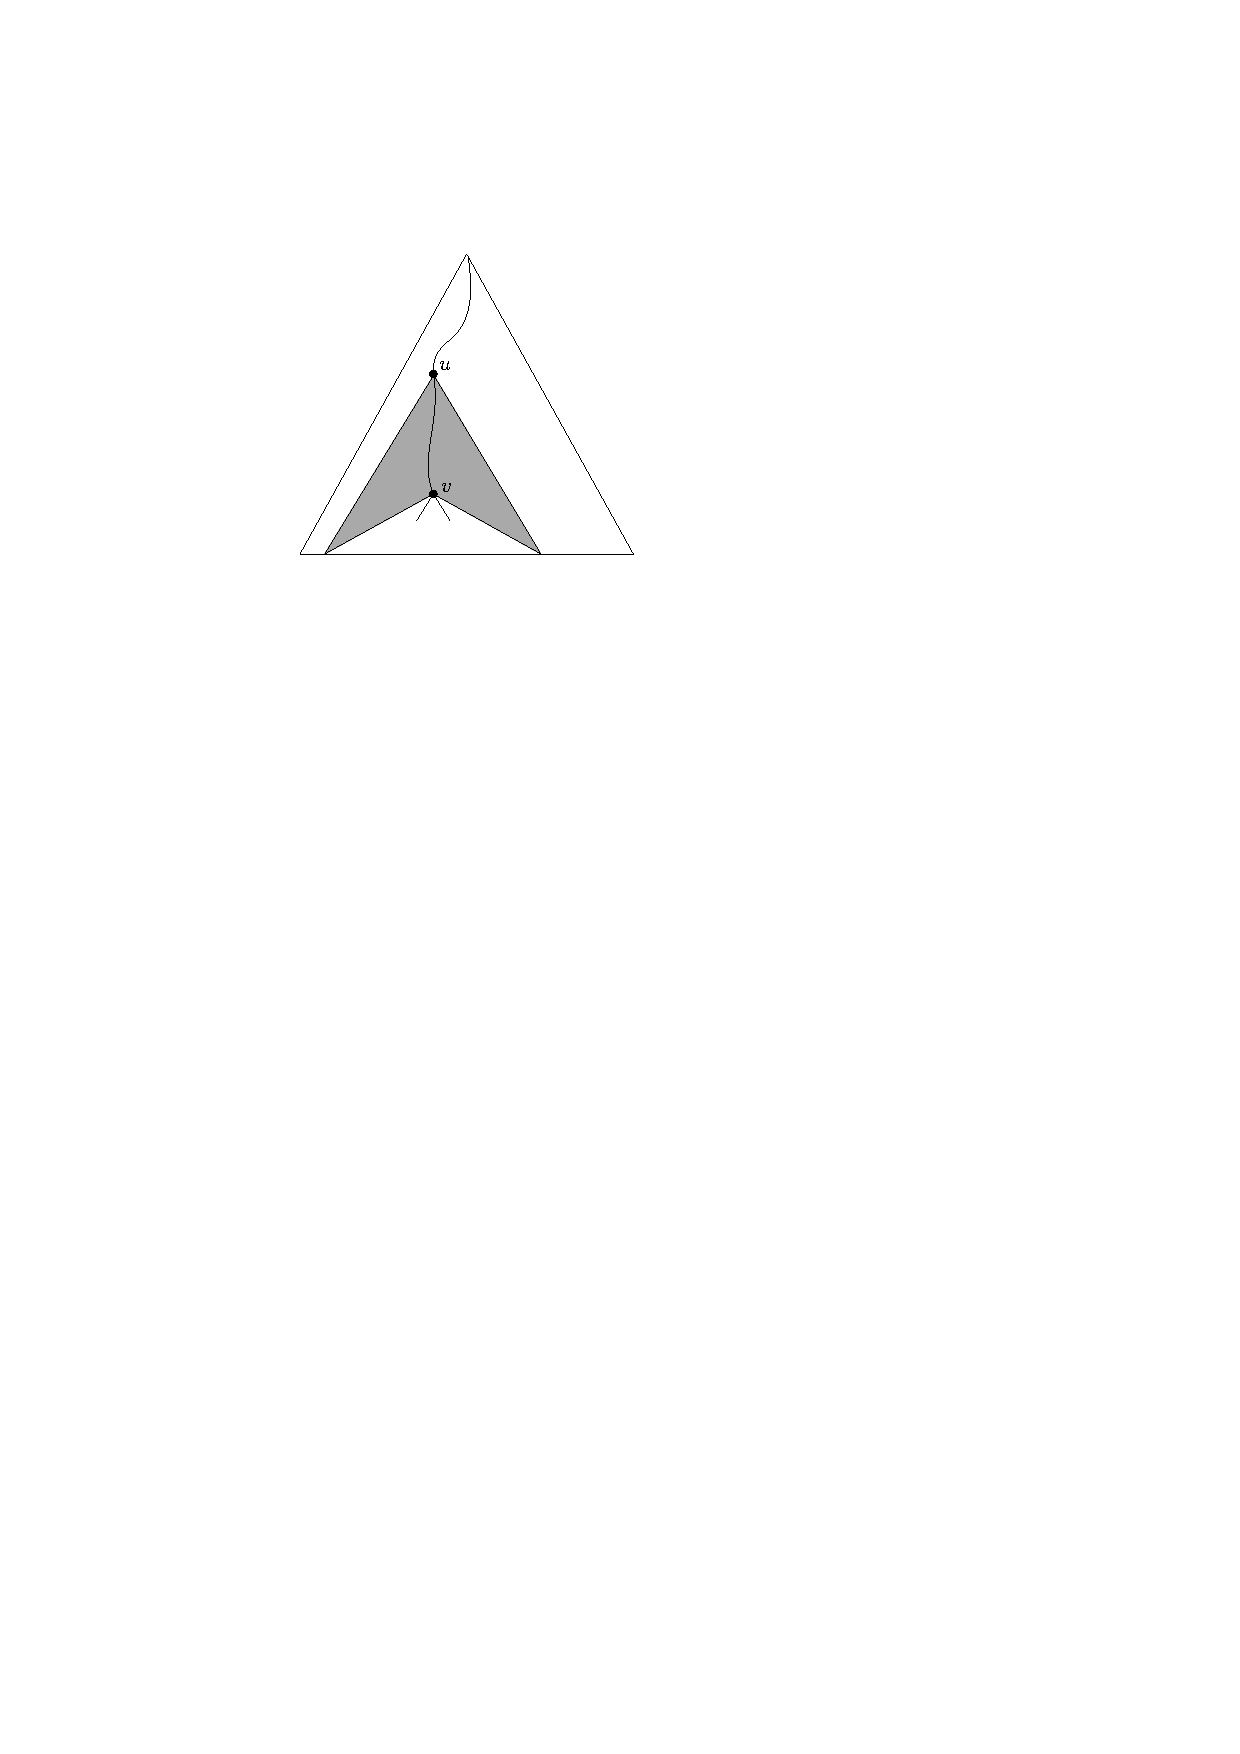
\includegraphics[scale=0.7]{fragment}}
%\end{figure}
 
\subsection{Preprocessing fragments} \label{Pre-Processing Fragments}
We now would like to preprocess the fragments, so that for any two nodes $u_{1}$ and $u_{2}$ in the same fragment we know
if $d(u_1,u_2)\geq\lambda$ or $d(u_1,u_2) \geq \frac{\lambda}{2}$, for any possible $\lambda$ specified in query time. 
This is done with the parametric search method by Frederickson as follows. We maintain an interval $[\lambda_1,\lambda_2)$ such that
$\lambda^{*}$ that we are searching for in the optimization problem is surely inside the interval, that is, $\lambda_{1}$ is feasible
while $\lambda_{2}$ is not. In the beginning, the interval is simply $[0,\infty)$. Then, we use $O(\log b)$ calls to the
linear-time feasibility test to further decrease the interval, so that most of the fragments have the property that any pairwise distance
(and also any pairwise distance multiplied by 2) inside is either smaller than $\lambda_{1}$ or larger or equal to $\lambda_{2}$.
A method of choosing which tests to perform to achieve this is the gist of Frederickson's method.

For each fragment, we construct an implicit representation of $O(b)$ matrices of total side length $O(b\log b)$, that are row- and column-sorted,
and any pairwise distance (and any pairwise distance multiplied by 2) inside is an entry in some matrix. This is done using the standard centroid 
decomposition as described in Appendix \ref{appendix constructing sorted matrices using centroid decomp.} in $O(n/b\cdot b\log b)=O(n\log b)$
total time. Then we use the following theorem:

\begin{theorem}[\cite{Frederickson1991}]\label{Frederickson's theorem}
Let  ${M_1, M_2, . . . , M_N}$ be a collection of sorted matrices in which matrix $M_j$ is of dimension $m_j \times n_j$, $m_j \leq n_j$, and $\sum_{j=1}^{N} m_j = m$.
Let p be nonnegative. The number of feasibility tests needed to discard all but at most $p$ of the elements is $O(\max \lbrace \log(\max_{j} \lbrace n_j \rbrace), \log(\frac{m}{p+1}) \rbrace)$, and the total running time exclusive of the feasibility tests is $O(\sum_{j=1}^{N} m_j \cdot \log (2n_j/m_j))$.
\end{theorem}
In our case, $m=b \log b \cdot \frac{n}{b} = n \log b$ and we set $p$ to be $n/b^2$. The theorem implies that we can use $O(\log b)$ feasibility tests and discard all but $n/b^2$ elements of the matrices.
We call fragments with the property that any pairwise distance (and any pairwise distance multiplied by 2) inside is either smaller than
$\lambda_{1}$ or larger or equal to $\lambda_{2}$ \text{inactive}, and all other fragments \textit{active}.
By the choice of parameters, we have at most $n/b^{2}$ active fragments (out of all $n/b$) and we also pay $O(n \log b)$ exclusive of the feasibility tests.
For an inactive fragment, we can now check if the distance between two nodes inside is at least $\lambda$ or $\lambda/2$ by
comparing it to $\lambda_{1}$.
This allows us to preprocess each inactive fragment in $O(b)$ time as follows:

\begin{enumerate}
\item\textbf{Reduce the fragment to a caterpillar:}\\
A fragment consists of the spine and the subtrees hanging off the spine. Because for any two nodes inside the fragment we can compare
their distance to $\lambda$ and $\lambda/2$, we can run our linear-time feasibility test on the subtrees hanging off the spine to obtain
the candidate and the certain node for each of them. The fragment is now reduced to a caterpillar with at most two leaves attached to each
spine node: the candidate node and the certain node.
\item\label{removing certain nodes}
\textbf{Find candidate nodes that cannot be taken into the solution:}\\
\label{removing impossible candidate nodes}
For every candidate node we want to find the nearest certain node. Then, we can compare their distance to $\lambda$ and remove the
candidate node if it cannot be taken. To find the nearest certain node, we first scan all nodes bottom-up (according to the natural order
on the spine nodes they are attached to) and compute for each of them the nearest certain node below it. Then, we repeat the scan
in the other direction to compute the nearest certain node above. This gives us, for every candidate node, the nearest certain node above
and below. We delete all candidate nodes for which one of these distances is smaller than $\lambda_{1}$.
We store the certain node nearest to the root, the certain node nearest to the hole and the total number of certain nodes,
and from now on ignore certain nodes and only deal with the remaining candidate nodes.
\item\label{making distances from the root monotone}
\textbf{Prune leaves to make their distances to the root non-decreasing:}\\
Let the $i$-th leaf, $u_{i}$, be connected with an edge of length $y_{i}$ to a spine node at distance $x_{i}$ from the root,
and order the leaves so that $x_{1}<x_{2}<\ldots<x_{s}$. See Figure~\ref{fig:pruning} in the appendix.
Note that $y_{i}<\frac{\lambda_{1}}{2}$, as otherwise $u_{i}$ would be a certain node.
Suppose that $u_{i-1}$ is farther from the root than $u_i$ (i.e.,
$x_{i-1}+y_{i-1} > x_i+y_i$), then:
$$d(u_{i},u_{i-1}) = x_i-x_{i-1}+y_i+y_{i-1} = x_{i} + y_{i} - x_{i-1} + y_{i-1} < 2y_{i-1} < \lambda_1.$$
Therefore an optimal solution cannot contain both $u_{i}$ and $u_{i-1}$. We claim that if the solution contains
$u_{i}$ then it can be replaced with $u_{i-1}$. To prove this, it is enough to argue that
$u_{i-1}$ is farther away from any node above it than $u_i$, and $u_i$ is closer to any node below it than $u_{i-1}$.
Consider a node $u_{j}$ that is above $u_{i-1}$ (so $j<i-1$), then:
$$d(u_j,u_{i-1}) - d(u_j,u_{i}) = y_{i-1}-(x_i-x_{i-1})-y_i = x_{i-1}+y_{i-1}-(x_i+y_i) > 0.$$
Now consider a node $u_{j}$ that is below $u_{i}$ (so $j>i$), then:
$$d(u_j,u_{i-1}) - d(u_j,u_{i}) = y_{i-1}+(x_i-x_{i-1})-y_i > 2(x_i-x_{i-1}) > 0.$$
So in fact, we can remove the $i$-th leaf from the caterpillar if $x_{i-1}+y_{i-1} > x_i+y_i$.
To check this condition efficiently, we scan the caterpillar from top to bottom while maintaining the most recently processed non-removed leaf.
The whole scan takes linear time in the number of candidate nodes and ensures that the distances of the
remaining leaves from the root are non-decreasing.

\item \label{making distances from the hole monotone}
\textbf{Prune leaves to make their distances to the hole non-increasing:}\\
This is done as in the previous step, except that we scan in the other direction.
\item\label{precompute for any candidate node}\textbf{Precompute for any candidate node with respect to the hole:}\\
We call $u_{1},u_{2},\ldots,u_{i}$ a {\em prefix} of the caterpillar and, similarly, $u_{i+1},u_{i+2}, \ldots,u_{s}$ a {\em suffix}.
For every possible prefix, we would like to precompute the result of running the linear-time feasibility
test on that prefix. In Section~\ref{sec:feasibility test} we will show that, in fact, this is enough to efficiently
simulate running the linear-time feasibility test on the whole subtree rooted at $r$ if we know the candidate
and the certain node w.r.t. the hole. Consider running the feasibility test on $u_{1},u_{2},\ldots,u_{i}$.
Recall that its goal is to choose as many nodes as possible, and in case of a tie to maximize the distance of the
nearest chosen node to $r$. Due to distances of the leaves to $r$ being non-decreasing, it is clear that
$u_{i}$ should be chosen. Then, consider the largest $i'<i$ such that $d(u_{i'},u_{i})\geq \lambda$ (recall that
such a test is actually done by comparing to $\lambda_{1}$). Due to distances of the leaves to the hole
being non-decreasing, nodes $u_{i'+1},u_{i'+2},\ldots,u_{i-1}$ cannot be chosen and furthermore $d(u_{j},u_{i})\geq \lambda$
for any $j=1,2,\ldots,i'$. Therefore, to continue the simulation we should repeat the reasoning for $u_{1},u_{2},\ldots,u_{i'}$.
This suggest the following implementation: scan the caterpillar from top to bottom and store, for every prefix $u_{1},u_{2},\ldots,u_{i}$,
the number of chosen nodes, the certain node and the candidate node. While scanning we maintain $i'$ in amortized constant time per $i$,
it is easy to see that after increasing $i$ we have to keep increasing $i'$ as long as $d(u_{i},u_{i'})<\lambda$.
To store the information for the current prefix, we copy the already computed information for $u_{1},u_{2},\ldots,u_{i'}$
and increase the number of chosen nodes by one. Then, if the candidate node is set to NULL and $d(r,u_{i})<\lambda/2$
we set the candidate node to $u_{i}$, and else if the certain node is set to NULL we set the certain node to $u_{i}$.
\end{enumerate}

\subsection{Feasibility test}
\label{sec:feasibility test}

The sublinear feasibility test processes the tree bottom-up. For every fragment with root $r$, we would like to simulate running the
linear-time feasibility test on the subtree rooted at $r$ to compute: the number of chosen nodes, the candidate node, and the certain
node. We assume that we already have such information for the fragment rooted at the hole of the current fragment, if any.
If the current fragment is active, we process it naively in $O(b)$ time (note that now we are given $\lambda$, and hence are
able to run the linear-time feasibility test). If the current fragment is inactive, we would like to process it in $O(\log b)$ time.
This can be seen as attaching the hole as another spine node to the corresponding caterpillar, and then executing steps
(\ref{removing certain nodes})-(\ref{precompute for any candidate node}).

We start by considering the case where there is no candidate node w.r.t. the hole. Let $v$ be the certain node w.r.t. the hole.
Because distances of the leaves from the hole are non-increasing,  we can compute the prefix of the caterpillar consisting of
leaves that can be chosen by binary searching for the largest $i$ such that $d(v,u_{i})\geq \lambda$. Then, we retrieve and return the result
stored for $u_{1},u_{2},\ldots,u_{i}$ (after increasing the number of chosen nodes and, if the certain node is set to NULL, updating it to $v$).

Now let the candidate node w.r.t. the hole be $u$. We start with binary searching for $i$ as explained above. Then,
we check if the distance between $u$ and the certain node nearest to the hole is smaller than $\lambda$ or
$d(u_{i},r)>d(u,r)$, and if so return the result stored for $u_{1},u_{2},\ldots,u_{i}$. Then, again because distances of the leaves
to the hole are non-increasing, we can binary search for the largest $i'\leq i$ such that $d(u_{i'},u)\geq \lambda$
(note that this also takes care of pruning leaves $u_{k}$ that are closer to the hole than $u$).
Finally, we retrieve and return the result stored for $u_{1},u_{2},\ldots,u_{i'}$ (after increasing the number of chosen nodes
and possibly updating the candidate and the certain node).

We process every inactive fragment in $O(\log b)$ and every active fragment in $O(b)$ time, so the total time is
$O(\frac{n}{b} \cdot \log b) + O(\frac{n}{b^2} \cdot b) = O(\frac{n}{b}\cdot \log b)$.

\subsection{\texorpdfstring{\boldmath$O(n\log\log n)$}{O(nloglogn)} Time Algorithm} 

The general idea of the algorithm is to use the heavy path decomposition to solve the optimization  problem
with $O(\log^{2}n)$ calls to the feasibility test. The {\em heavy edge} of a non-leaf node of the tree is the edge leading to the child
with the largest number of descendants. These heavy edges define a decomposition of the nodes into heavy paths. Each heavy
path $p$ starts with a head $\head(p)$ and ends with a tail $\tail(p)$ such that $\tail(p)$ is a descendant of $\head(p)$,
and its depth is the number of heavy paths $p'$ such that $\head(p')$ is an ancestor of $\head(p)$. The depth of any heavy path is 
$O(\log n)$~\cite{Sleator1983}.

We process all heavy paths at the same depth together while maintaining an interval $[\lambda_{1},\lambda_{2})$ such that
$\lambda_{1}$ is feasible while $\lambda_{2}$ is not, that is, the sought $\lambda^{*}$ belongs to the interval.
The goal of processing the heavy paths at depth $d$ is to further shrink the interval so that the result of running the feasibility
test on any subtree rooted at $\head(p)$ is the same for any $\lambda\in[\lambda_{1},\lambda_{2})$ and therefore can
be already determined, for any heavy path $p$ at depth $d$. We start with the heavy paths of maximal depth and terminate
with $\lambda^{*}=\lambda_{1}$ after having determined the result of running the feasibility test on the whole tree.
Let $n_{d}$ denote the total size of all heavy paths at depth $d$.

Let $n_{d}$ denote the total size of all heavy paths at depth $d$. For every such heavy path we construct a caterpillar by replacing
every hanging off subtree by the certain and the candidate node (this is possible, because we have already determined the result of
running the feasibility test on that subtree). To account for the possibility of including a node of the heavy path in the solution,
we attach an artificial leaf connected with an zero-length edge to every such node.
The caterpillar is then pruned similarly to steps (\ref{removing impossible candidate nodes})-(making distances from the hole monotone)
from Section~\ref{Pre-Processing Fragments}, except that after having found the nearest certain node for every candidate
node we cannot simply compare their distance to $\lambda_{1}$. Instead, we create an $1\times 1$ matrix storing the relevant
distance for every candidate node. Then, we apply Theorem~\ref{Frederickson's theorem} with $p=0$ to the obtained set of
$O(n_{d})$ matrices of dimension $1\times 1$. This allows us to determine, using only $O(\log n)$ feasibility tests and
$O(n_{d})$ time exclusive of the feasibility tests, which distances are larger than $\lambda^{*}$, so that we can prune
the caterpillars and work only with the remaining candidate nodes. Then, for every caterpillar we create a row- and column-sorted matrix
storing pairwise distance between its leaves. By applying Theorem~\ref{Frederickson's theorem} with $p=0$ on the obtained set of
square matrices of total side length $O(n_{d})$ we can determine, with $O(\log n)$ feasibility tests and $O(n_{d})$ time
exclusive of the feasibility tests, which distances are larger than $\lambda^{*}$. This allows us to run the bottom-up
procedure described in Section~\ref{linear F.T.} to produce the candidate and the certain node for every subtree rooted
at $\head(p)$, where $p$ is a heavy path at depth $d$.

All in all, for every $d$ we spend $O(n_{d})$ time and execute $O(\log n)$ feasibility tests. Summing over all depths $d$,
this is $O(n)$ plus $O(\log^{2}n)$ calls to the feasibility test. Setting $b=\log^{2}n$, the total time is thus $O(n+n\log\log n+\frac{n}{\log^{2}n}\cdot\log\log n\cdot \log^{2}n)=O(n\log\log n)$.

\section{A Linear Time Algorithm for the Dispersion Problem}
\label{sectionLinear}

To accelerate the $O(n\log\log n)$ time algorithm, we construct a hierarchy of feasibility tests by partitioning the input tree
into larger and larger fragments, starting from the linear-time implementation described in Section~\ref{linear F.T.}. 
Given a feasibility test with $O(\frac{n}{b^4}\log b)$ query-time, we show how to obtain in $O(\frac{n}{b})$ time a feasibility test with
$O(\frac{n}{(2^b)^{4}}\log (2^b))$ query-time.
After $\log ^*n$ iterations requiring a total of $O(n)$ time, we obtain a feasibility test with $O(\frac{n}{\log ^4n} \cdot \log \log n)$ query-time
which we use to solve the dispersion optimization problem in $O(n)$. 

There are multiple technical difficulties that need to be overcome in order to keep the preprocessing time $O(\frac{n}{b})$.
We must make each partition into fragments a refinement of the previous one, i.e. the fragments of the $(\ell+1)$-th partition (called large fragments)
are composed of fragments of the $\ell$-th partition (called small fragments). We believe that this simple micro-macro variant is of independent interest. 
Further, we cannot afford to touch every node of every fragment at every decomposition level. Therefore, we take a closer look at how a (large) fragment decomposes into smaller fragments. 
We show that a large fragment can be reduced to a concatenation of small caterpillars, each corresponding to a small fragment that we have already preprocessed. We then carefully tailor these small caterpillars while reusing the results of their preprocessing. We show that this tailoring amortizes to $O(n)$ over all decompositions. Due to space constraints, the full description of the algorithm is in Appendix \ref{appendix linear algorithm for the dispersion optimization problem}.

\section{The Weighted Dispersion Problem}\label{section:weighted}
We now consider the weighted variant of the dispersion problem, in which the edges have lengths and the nodes have weights. Recall that $f(P)=\min_{u,v\in P} \{d(u,v)\}$. The weighted dispersion problems are defined as follows.
\begin{itemize} 
\item {\em The Weighted Dispersion Optimization Problem.} Given a tree with non-negative edge lengths, non-negative node weights, and a number $W$, find a subset of nodes $P$ of weight at least $W$, such that  $f(P)$ is maximized. 

\item {\em The Weighted Dispersion Decision Problem.} Given a tree with non-negative edge lengths, non-negative node weights, a number $W$, and a number $\lambda$, find a subset of nodes  $P$ of weight at least $W$, such that $f(P)\geq\lambda$, or declare no such subset exists. 
\end{itemize}


In this section we present an $O(n\log n)$ time algorithm for the weighted decision problem. A matching lower bound follows by a reduction from the set disjointness problem (see Appendix \ref{appendix weighted f.t. lower bound}).
Using Frederickson's algorithm for finding the $k$-th longest path \cite{Frederickson1983} we can binary search over the possible values of $\lambda$ and solve the optimization problem with $O(\log n)$ calls to the $O(n \log n)$ time feasibility test, and $O(n\log^{2}n)$ time overall.

Similarly to the unweighted case, we would like to compute for each node of the tree, the subset of nodes $P$ in its subtree  s.t. $f(P) \geq \lambda$ and $W(P)$ is maximized. We compute this by going over the nodes of the tree bottom-up. Previously, the situation was simpler, as for any subtree we had just one candidate node (i.e., a node that may or may not be in the optimal solution for the entire input tree). This was true because nodes had uniform weights. Now however, there could be many candidates in a subtree, as the certain nodes are the ones that are at distance at least $\lambda$ from the root (and not $\frac{\lambda}{2}$ as in the unweighted case).

Let $P$ be a subset of the nodes in the subtree rooted at $v$, and let $h$ be the node in $P$ for which $d(h,v)$ is minimized. We call $h$ the {\em closest chosen node} in $v$'s subtree. In our weighted feasibility test, $v$ will store an optimal solution $P$ for each possible value of $d(h,v)$ (up to $\lambda$, since if the closest chosen node is farther, it does not affect nodes outside the subtree). That is, a subset of nodes $P$ in $v$'s subtree of maximum weight $W(P)$ s.t. the closest chosen node is at distance {\em larger or equal} to $d(h,v)$ from $v$, and $d(x_1,x_2) \geq \lambda$ for every  $x_1,x_2\in P$. 
The values $W(P)$ can be viewed as a monotone polyline, since the weight of $P$ only decreases as the distance of the closest chosen node increases (from zero to $\lambda$). The weight of $P$ can only change at certain points called the {\em breakpoints} of the polyline. Each point of the polyline is a key-value pair, where the key is $d(h,v)$ and the value is $W(P)$. We store with each breakpoint the value of the polyline between it and the next breakpoint. I.e. for some pair of consecutive breakpoints with keys $a$ and $a+b$, we store in the first breakpoint the value of the polyline in the interval $[a,a+b)$. As a special case, the first breakpoint stores the value of the polyline in the interval $(0,a)$ (where $a$ is the key of the second breakpoint), and we store the value for key zero separately. The representation of a polyline consists only of its breakpoints.

%\begin{figure}[h]
%\begin{center}
%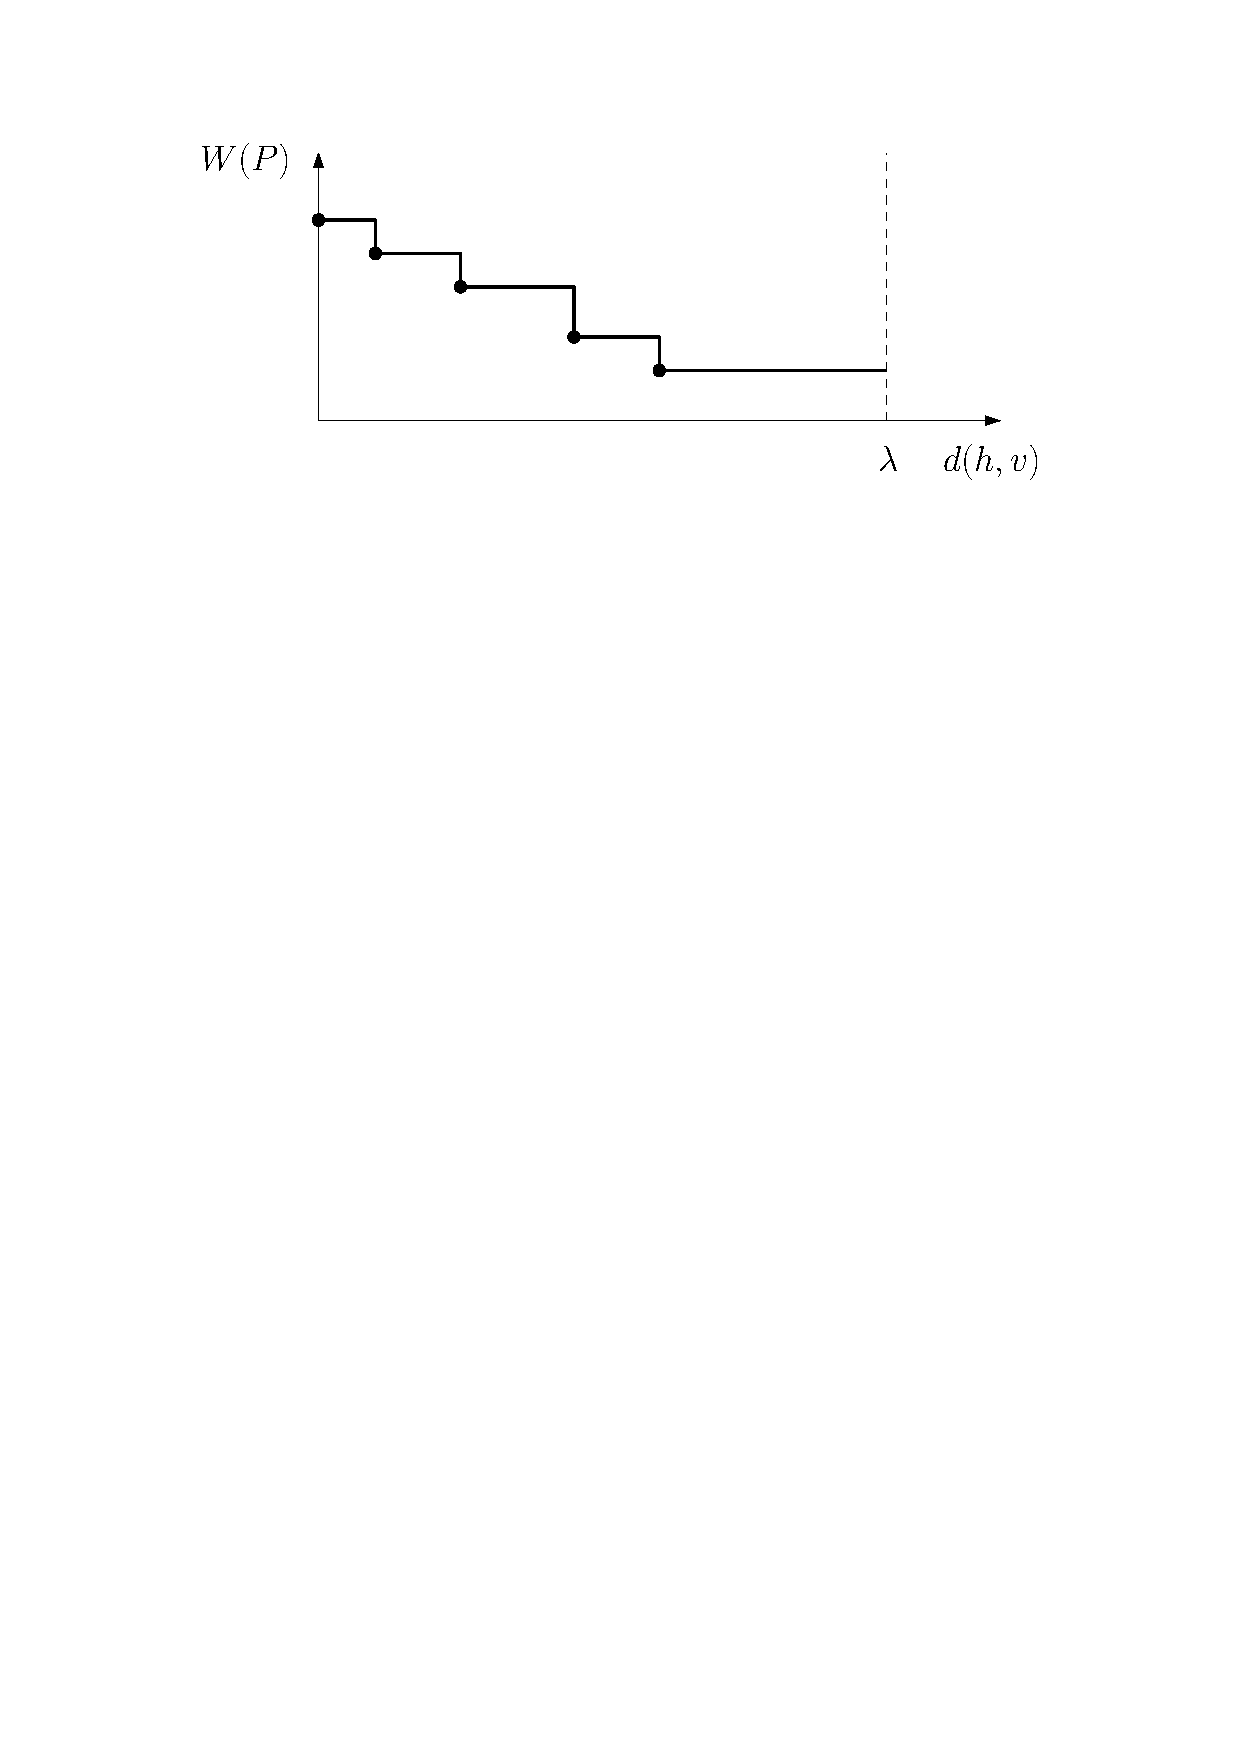
\includegraphics[scale=0.55]{polyline}
%\end{center}
%\caption{The polyline represents the weight of the optimal solution $P$ as a function of the distance of the closest chosen node in the subtree. %$v$ is the root of the subtree, and $h$ is the chosen node closest to $v$ in its subtree. 
%The weight of $P$ only decreases at certain points called breakpoints (in bold). Each breakpoint stores the value in the interval between itself and the next breakpoint.
%\label{figure of a polyline}}
%\end{figure}


The algorithm computes such a polyline for the subtrees rooted at all the nodes of the tree. As we have mentioned, this computation is done bottom-up, and so in each step of the algorithm we compute the polyline for a subtree rooted at some node $v$, assuming that we have already computed the polylines for the subtrees rooted at $v$'s children. We will show how to achieve this step in time $O(x \log (\frac{2y}{x}))$, where $x$ is the number of breakpoints in the polyline with fewer breakpoints, and $y$ the number of breakpoints in the other polyline\footnote{For the same reasoning as in the unweighted case, we assume w.l.o.g. that the input tree is binary.}. This sums up to $O(n \log n)$ overall.


When constructing a polyline, we need to consider several cases, as the closest chosen node $h$ in the subtree of $v$ could be $v$ itself, or it could be in the subtree of one of $v$'s children. This means that for any key $d(h,v)$ in the polyline, the value for that key can represent a solution $P$ in which $h$ is in the subtree rooted $v$'s left child, or in the subtree rooted $v$'s right child, or it could be $v$ itself.


\medskip \noindent {\bf Constructing a polyline.} We now present a single step of the algorithm. We postpone the discussion of the data structure used to store the polylines for now, and first describe how to obtain the polyline of $v$ from the polylines of its children. Then, we state the exact interface of the data structure that allows executing such a procedure efficiently, show how to implement such an interface, and finally analyze the complexity of the resulting algorithm.

If $v$ has only one child $u$, then we build $v$'s polyline by querying $u$'s polyline for the case that $v$ is in the solution (i.e. query $u$'s polyline with distance of the closest chosen node being $\lambda-d(v,u)$), and add to this value the weight of $v$ itself. We then construct the polyline by taking the value we got (which will be the value for $d(h,v)=0$) and merging it with the polyline computed for $u$, shifted to the right by $d(v,u)$ (since we now measure the weight of the solution as a function of the distance of the closest chosen node to $v$, not to $u$). The value between zero and $d(v,u)$ will be the same as the value of the first interval in the polyline constructed for $u$, so the shift is actually done by increasing the keys of all but the first breakpoint by $d(v,u)$.

If $v$ has two children, denote its left child by $u_1$ and its right child by $u_2$. We have two polylines that represent the solutions inside the subtrees rooted at $u_1$ and $u_2$ (denoted by $p_1$ and $p_2$, respectively), and we want to create the polyline for the subtree rooted at $v$ (denoted by $p$). Denote the number of breakpoints in $p_1$ by $x$ and the number of breakpoints in $p_2$ by $y$. Assume w.l.o.g. that $x \leq y$.

We begin with computing the value of $p$ for key zero. Consider the case where $v$ is in the solution (i.e., $h=v$). In this case we query $p_1$ and $p_2$ for their values with keys $\lambda - d(v,u_1)$ and $\lambda - d(v,u_2)$ respectively (if one of these is negative, we take zero instead), and add them together with the weight of $v$. Another possible case is that there is a better solution (i.e. a subset with greater weight) for the subtree rooted at $v$, where $v$ is not included in the solution. For this we need to check, after constructing the rest of the polyline, whether the value stored at the first breakpoint is greater than the value we computed for the case $v$ is chosen. If so, we store the value of the first breakpoint also as the value for key zero.

We now show how to construct the rest of the polyline $p$. Notice that we need to maintain that $d(h_1,h_2) \geq \lambda$ (where $h_1$ is the closest chosen node in $u_1$'s subtree and $h_2$ is the closest chosen node in $u_2$'s subtree). We proceed in two steps, each computing half of the polyline $p$.

\subsection{Constructing the second half of the polyline.}\label{subsection constructing the second half of the polyline} We start by constructing the second half of the polyline, where $d(h,v) \geq \frac{\lambda}{2}$. In this case we query both polylines with the same key, since $d(h_1,v) \geq \frac{\lambda}{2}$ and $d(h_2,v) \geq \frac{\lambda}{2}$ implies that $d(h_1,h_2) \geq \lambda$. The naive way to proceed would be to iterate over the second half of both polylines in parallel, and at every point sum the values of the two polylines to get the value of the new polyline. This would not be efficient enough. Therefore, instead of iterating over $p_2$ (the larger polyline) we iterate over all the breakpoints in the second half of $p_1$ (the smaller polyline). These breakpoints induce intervals of $p_2$. For each of these intervals we increase the value of $p_{2}$ by the value in the interval in $p_1$ (see Figure~\ref{figure of constructing the second half of the polyline}). For this we might need to insert some of the breakpoints from $p_1$ if there is no such breakpoint already in $p_2$. Thus, we have obtained the second half of the monotone polyline $p$ by modifying the second half of the monotone polyline $p_{2}$.

%\begin{figure}[h]
%\begin{center}
%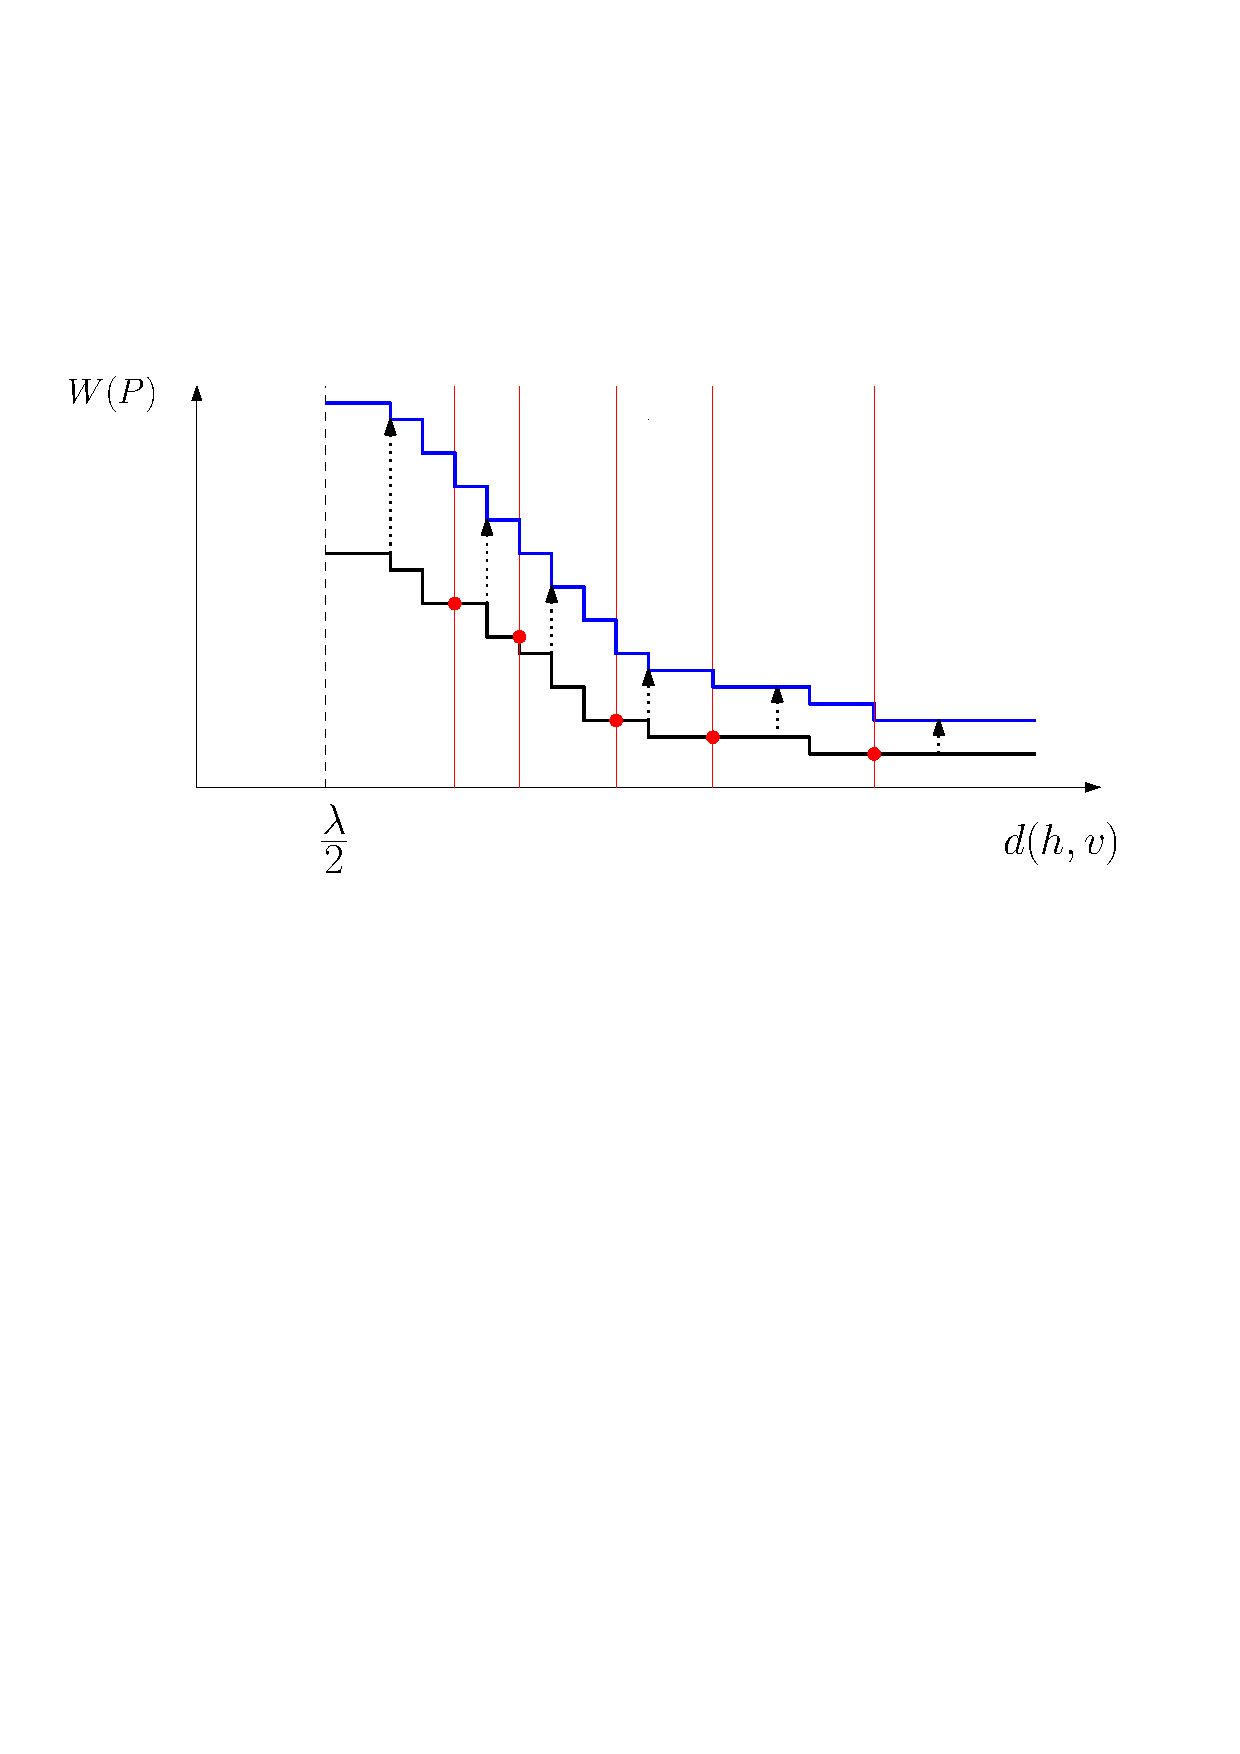
\includegraphics[scale=.55]{new_polyline_second_half}
%\end{center}
%\caption{Constructing the second half of the polyline $p$ (in blue). The black polyline is $p_2$. The breakpoints inserted from $p_1$ are in red. In each interval (between consecutive red lines) we raise the polyline by the value in $p_1$.
%\label{figure of constructing the second half of the polyline}}
%\end{figure}

\subsection{Constructing the first half of the polyline.} We need to consider two possible cases: either $d(h_1,v) < d(h_2,v)$ (i.e. the closest chosen node in $v$'s subtree is inside $u_1$'s subtree), or $d(h_1,v) > d(h_2,v)$ (note that in this half of the polyline $d(h,v)<\frac{\lambda}{2}$, and therefore $d(h_1,v) \neq d(h_2,v)$). For each of the two cases we will construct the first half of the polyline, and then we take the maximum of the two polylines at every point, in order to have the optimal solution for each key.

\medskip \noindent {\bf Case I: \boldmath$d(h_1,v) < d(h_2,v)$.} Since we are only interested in the first half of the polyline, we know that $d(h_1,v) < \frac{\lambda}{2}$. Since $d(h_2,v) +d(h_1,v)\geq \lambda$ we have that  $d(h_2,v) > \frac{\lambda}{2}$. Again, we cannot afford to iterate over the breakpoints of $p_2$, so we need to be more subtle.

We start by splitting $p_1$ at $\frac{\lambda}{2}$ and taking the first half (denoted by $p_1'$). We then split $p_2$ at $\frac{\lambda}{2}$ and take the second half (denoted by $p_2'$). Consider two consecutive breakpoints of $p_1'$ with keys $x$ and $x+y$. We would like to increase the value of $p_1'$ in the interval $[x,x+y)$ s.t. the new value is the maximal weight of a valid subset of nodes \emph{from both subtrees} rooted at $u_1$ and $u_2$, s.t. $x \leq d(h_1,v)<x+y$. Therefore $d(h_2,v)>\lambda-x-y$. $p_2'$ is monotonically decreasing, and so we query it at $\lambda-x-y+\epsilon$, and increase by the resulting value.

This process might result in a polyline which is not monotonically decreasing, because as we go over the intervals of $p_1'$ from left to right we increase the values there more and more.
To complete the construction, we make the polyline monotonically decreasing by scanning it from $\frac{\lambda}{2}$ to zero and deleting unnecessary breakpoints. This takes $O(x)$ time.
Note that in the above description we have assumed that we have access to the original data structure representing $p_{2}$, but this structure has been already modified to obtain the second half of $p$. However, we started with computing the second half of $p$ only to make the description simpler, and we can simply start with the first half.

%\begin{figure}[h]
%\begin{center}
%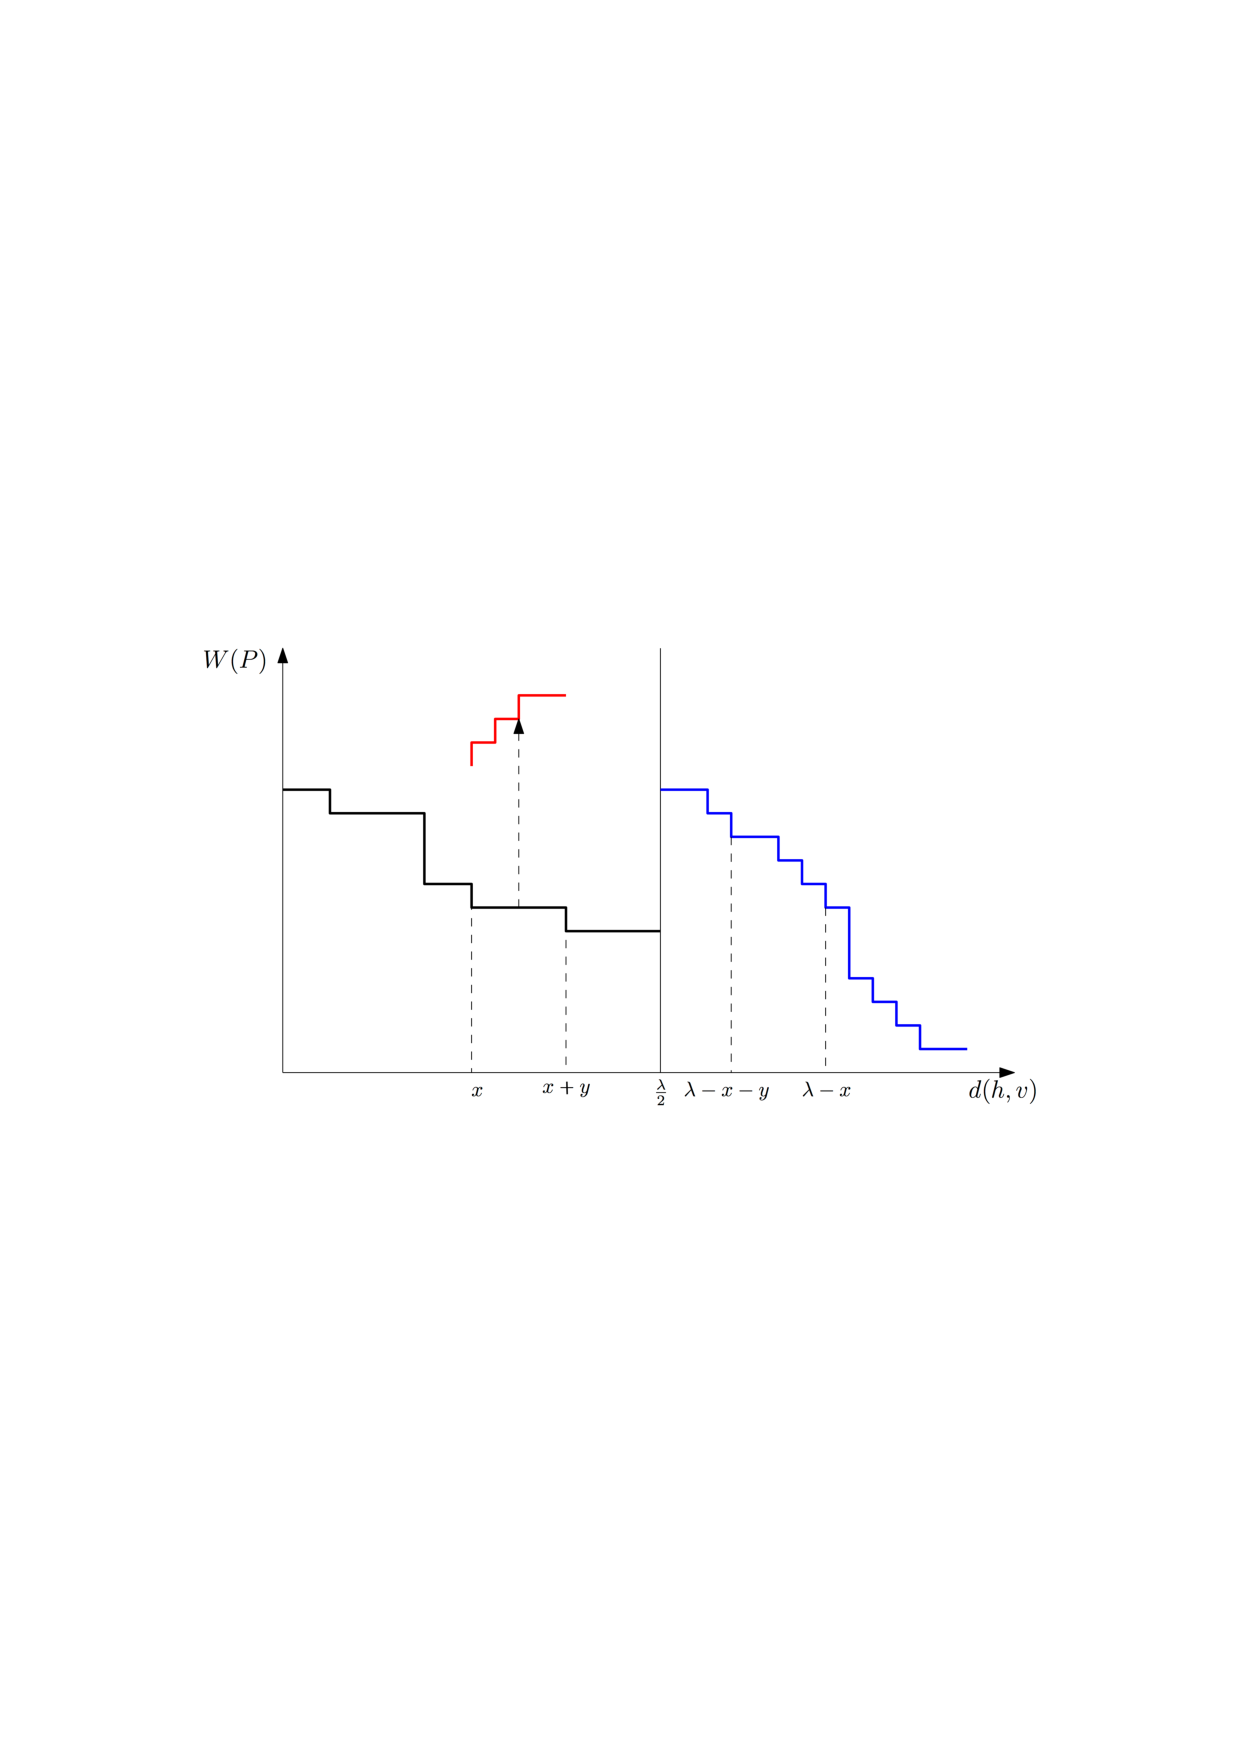
\includegraphics[scale=0.8]{polyline_first_half_construction_case1}
%\end{center}
%\caption{Case I of constructing the first half of the polyline. $p_1'$ (in black) is the first half of $p_1$, $p_2'$ (in blue) is the second half of $p_2$. The red polyline is the result of increasing the values of $p_1$ in the interval between $x$ and $x+y$ by the appropriate values of $p_2'$. The result is non-monotone, so we actually need to increase by the maximal value, i.e. the value of $p_2'$ at $\lambda-x-y+\epsilon$.\label{figure of constructing the first half of the polyline case 1} 
%}
%\end{figure}

\medskip \noindent {\bf Case II: \boldmath$d(h_1,v) > d(h_2,v)$.}
Symmetrically to the previous case, we increase the values in the intervals of $p_2$ induced by the breakpoints of $p_1$ by the appropriate values of $p_{1}$ (similarly to what we do in subsection \ref{subsection constructing the second half of the polyline}). Again, the resulting polyline may be non-monotone, but this time we cannot solve the problem by scanning the new polyline and deleting breakpoints, since there are too many of them. Instead, we go over the breakpoints of the second half of $p_1$ from right to left. For each such breakpoint  with key $x$, we find the {\em value} of key $\lambda - x$ in the new polyline. These are the points where we might have increased the value of $p_2$. Denote this value by $y$. We then query the new polyline with a \emph{value predecessor} query: this returns the breakpoint   with the largest key s.t. its key is smaller than $\lambda - x$ and its value is at least $y$. 
%
If this breakpoint exists, then the values of the new polyline between its successor breakpoint and $\lambda - x$ should all be $y$ (i.e. we delete all breakpoints in this interval except for the first one whose value we set to $y$). % (if it is the predecessor of $x$ in the list of breakpoints, then this is already the case).
If it does not exist, then the values between zero and $\lambda - x$ should be $y$ (i.e. we delete all the previous breakpoints). 
This ensures that the resulting polyline is monotonically decreasing. 
See  Figure~\ref{figure of the second case in the construction of the first half of the polyline}.



%\begin{figure}[h]
%\begin{center}
%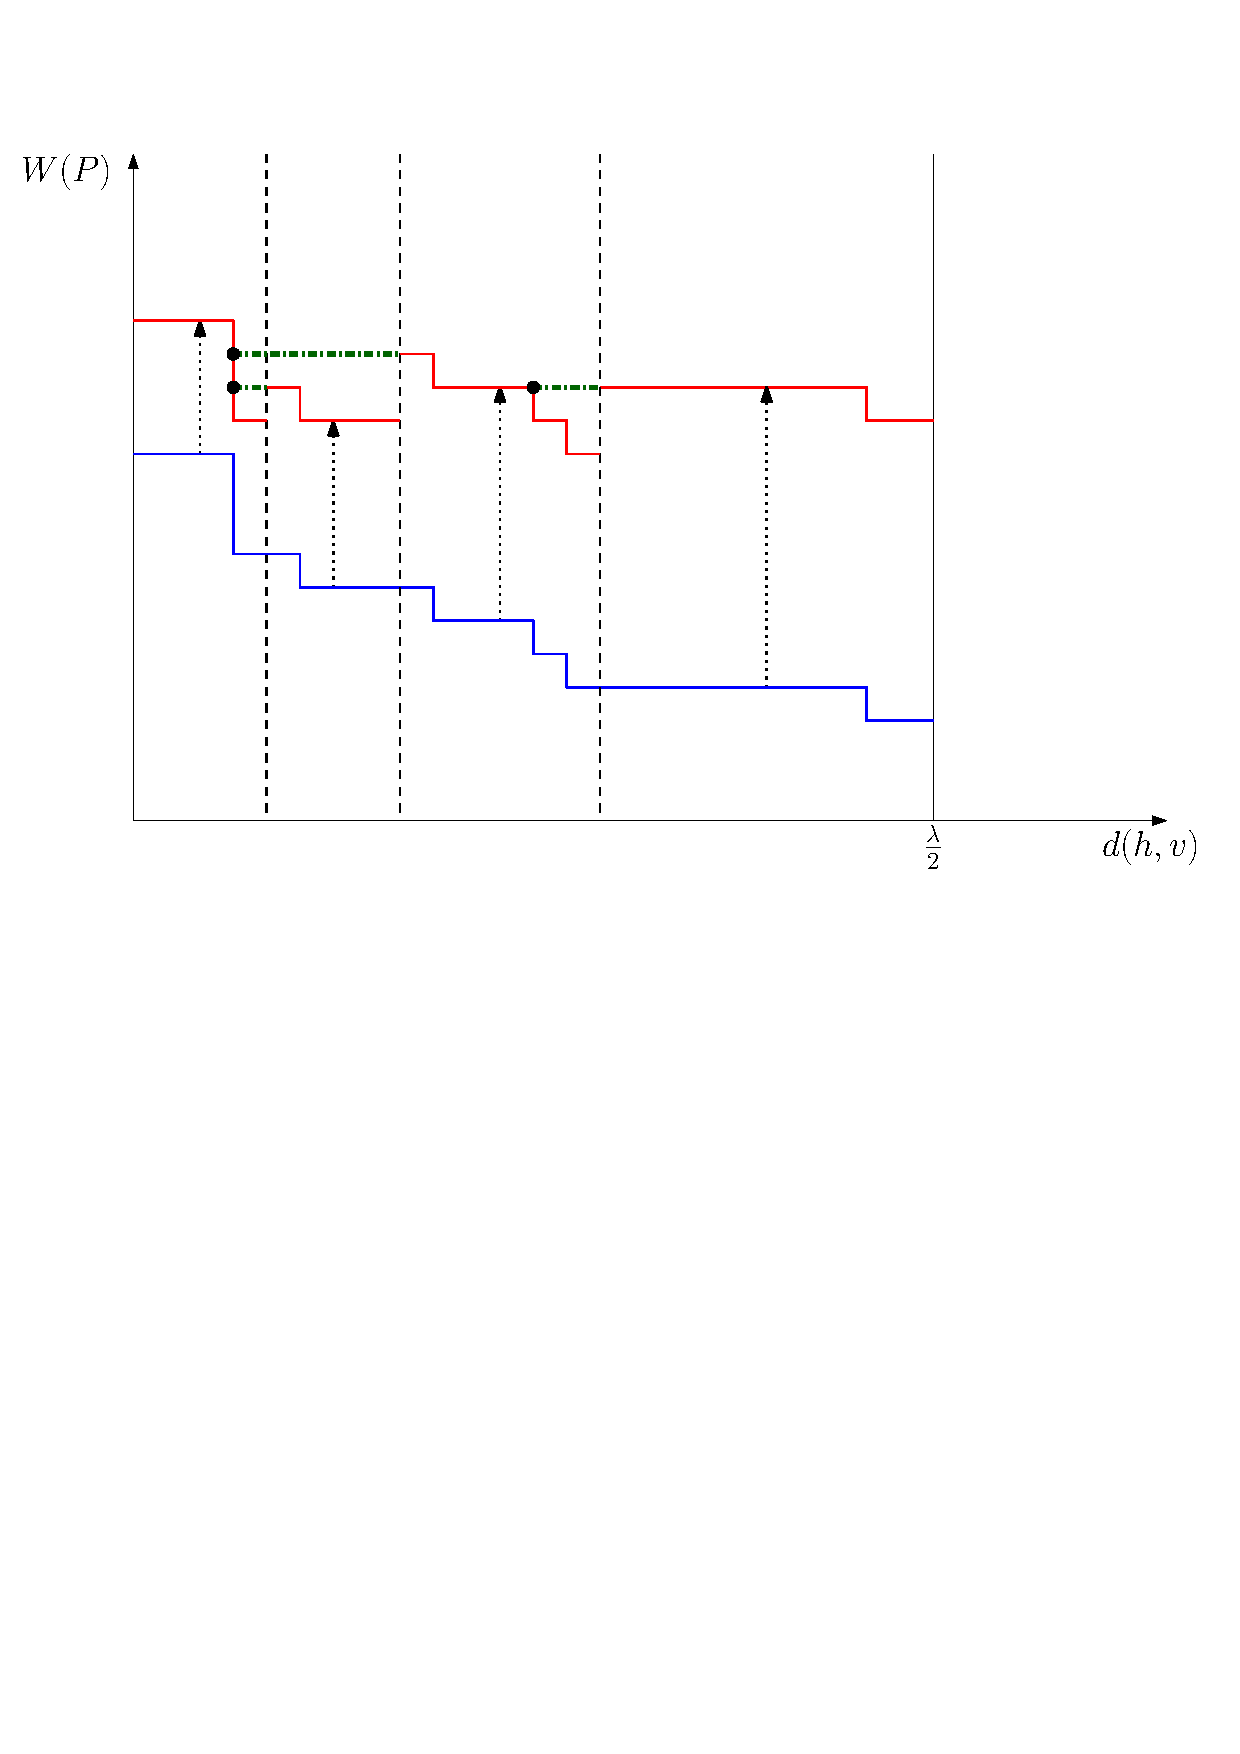
\includegraphics[scale=0.6]{polyline_first_half_construction_case2}
%\end{center}
%\caption{Case II of constructing the first half of the polyline. The first half of $p_2$ is in blue. The vertical black dashed lines are the breakpoints of $p_1$. We increase the values of $p_{2}$ and obtain the red polyline, which is not monotone. To make it monotone, we delete all the breakpoints below the green intervals, which are found with value predecessor queries (the results of these queries are the bold points).\label{figure of the second case in the construction of the first half of the polyline}
%}
%\end{figure}

\medskip \noindent {\bf Merging cases I and II.}
We now need to build one polyline for the first half of the polyline, taking into account both cases. Let $p_a$ ($p_b$) denote the polyline we have constructed in case I (II) (so the number of breakpoint in $p_a$ is at most the number of breakpoints in $p_b$). We start by shifting $p_a$ and $p_b$ to the right by $d(v,u_1)$ and $d(v,u_2)$ respectively, because now measure the distance of $h$ from $v$, not from $u_1$ or $u_2$. 

We now need to take the maximum of the values of $p_a$ and $p_b$, for each key. We do this by finding the intersection points of the two polylines. Notice that since both polylines are monotonically decreasing, these intersections can only occur at (i) the breakpoints of $p_a$, (ii) at most one point between two consecutive breakpoints of $p_a$. We iterate over $p_a$ and for every pair of consecutive breakpoints, we check which polyline has the higher value at both points. If the answer for both points is the same, we carry on. Otherwise, there must be a single intersection point of the two polylines inside this interval. We find this intersection by running a value predecessor query on $p_b$, with the key being the right endpoint of the interval. After such computation, we know which polyline gives us the best solution for every point between zero and $\frac{\lambda}{2}$, and where are the intersection points where this changes. We can now build the new polyline by doing insertions and deletions in $p_b$ according to the intersection points: For every interval of $p_b$ defined by a pair of consecutive intersection points, we check if the value of $p_a$ is larger than the value of $p_b$ in the interval, and if so, delete all the breakpoints of $p_b$ in the interval, and insert the relevant breakpoints from $p_a$. The number of intersection points is linear in the number of breakpoints of $p_a$ which is $O(x)$, and so, the total number of interval deletions and insertions is also $O(x)$.

To conclude, the final polyline $p$ is obtained by concatenating the value computed for key zero, the polyline computed for the first half, and the polyline computed for the second half. 


\subsection{The polyline data structure} We now specify the data structure for storing the polylines. The required interface is:
\begin{enumerate}
\item \label{op1} Split the polyline at some key.
\item \label{op2} Merge two polylines (s.t. all the keys in one polyline are smaller than all keys in the other).
\item \label{op3} Retrieve the value of the polyline for a certain key $d(h,v)$.
\item \label{op4}Return a sorted list of the breakpoints of the polyline
\item \label{op5} Batched interval increase -- Given a list of disjoint intervals of the polyline, and a number for each interval, increase the values of the polyline in each interval by the appropriate number. Each interval is given by the keys of its endpoints.
\item \label{op6} Batched value predecessor -- Given a list of key-value pairs, $(k_i,v_i)$, find for each $k_i$, the maximal key $k_{i}'$, s.t. $k_{i}' < k_i$ and the value of the polyline at $k_{i}'$ is at least $v_i$.
\item \label{op7} Batched interval insertions -- Given a list of pairs of consecutive breakpoints in the polyline, insert between each pair a list of breakpoints.
\item \label{op8} Batched interval deletions -- Given a list of disjoint intervals of the polyline, delete all the breakpoints inside the intervals.
\end{enumerate}

We now describe the data structure we use for polylines, which will allow us to implement the above interface efficiently. We represent a polyline by storing its breakpoints in an augmented 2-3 tree, where the data is stored in the leaves. Each node of the tree stores a key-value pair, and we maintain the following property: the key of each breakpoint is the sum of the keys of the corresponding leaf and of all its ancestors, and similarly for the values. In addition, we store in each node the maximal key and the maximal value of a breakpoint that corresponds to a leaf in its subtree. We also store in each node the number of leaves in its subtree. We next describe the implementation of each operation.

 Operations~\ref{op1} and~\ref{op2} can use standard split and join procedures for 2-3 trees in logarithmic time. 
 Operation~\ref{op3} can be done by running a predecessor query and returning the value at the returned breakpoint in logarithmic time.
 Operation~\ref{op4} is done by an inorder traversal of the tree. 
Operations~\ref{op1}-\ref{op3} are performed only a constant number of times per step, and so their total cost is logarithmic (i.e. $O(\log x + \log y)$). Operation~\ref{op4} is also performed a constant number of times to iterate over the breakpoints of $p_{1}$ (in $O(x)$ time). The next four operations are more costly, since each of them is comprised of a batch of $O(x)$ operations on a tree of size $O(y)$. The input to all these four batched operations is assumed to be given in sorted order (by keys).


\medskip \noindent {\bf Operation~\ref{op5} -- batched interval increase.}
Consider the following implementation for Operation \ref{op5}. We iterate over the intervals, and for each of them, we find its left endpoint, and traverse the path from the left endpoint, through the lowest common ancestor (LCA), to the right endpoint.
The traversal is guided by the maximal keys stored at the nodes.\footnote{We need to maintain during the traversal the sum of all keys on the path from the root to the current node. This quantity can be easily maintained in constant time while moving to a child or the parent.}
While traversing the path from the left endpoint to the LCA (from the LCA to the right endpoint), we increase the value of every node hanging to the right (left) of this path. We also update the maximal value field in each node we reach (including the nodes on the path from the LCA to the root). Notice that if one of the endpoints of the interval is not in the structure, we need to insert it. We might also need to delete a breakpoint if it is a starting point of some interval and its new value is now equal to the value of its predecessor. This implementation would take time which is linear in the number of traversed nodes, plus the cost of insertions and deletions (whose number is linear in the number of intervals). Because the depth of a 2-3 tree of size $O(y)$ is $O(\log y)$, this comes up to $O(x \log y$). Such time complexity for each step would induce a running time of $O(n \log ^2 n)$ for the entire feasibilty test. 

We improve the running time by performing the operations on smaller trees. The operation therefore begins by splitting the tree into $O(x)$ smaller trees, each with $O(\frac{y}{x})$ leaves. This is done by recursively splitting the tree, first into two trees with $O(\frac{y}{2})$ leaves, then we split each of these trees into two trees with $O(\frac{y}{4})$ leaves, and so on, until we have trees of size $O(\frac{y}{x})$. We then increase the values in the relevant intervals using the small trees. For this, we scan the roots of the small trees, searching for the left endpoint of the first interval (by using the maximal key stored in the root of each tree). Once we have found the left endpoint of the interval, we check if the right endpoint of the interval is in the same tree or not (again, using the maximal key). In the first case, the interval is contained in a single tree, and can be increased in this tree in time $O(\log(\frac{y}{x}))$ using the procedure we have previously described. In the second case, the interval spans several trees, and so we need to do an interval increase in the two trees containing the endpoints of the interval, and additionally increase the value stored in the root of every tree that is entirely contained in the interval. We then continue to the next interval, and proceed in the same manner. 
%
Since the intervals are disjoint and we do at most two interval increases on small trees per interval, the total time for the increases in the small trees is $O(x \cdot \log (\frac{y}{x}))$. Scanning the roots of the small trees adds $O(x)$ to the complexity, leading to 
 $O(x \cdot \log (\frac{y}{x}) + x) = O(x \log (\frac{2y}{x}))$ overall for processing the small trees.

Before the operation terminates, we still need to merge the small trees back into one large tree. We do this using join operations, symmetrically to how we obtained the small trees by splitting. 

\begin{restatable}{lemmarestatable}{runningtimetoobtainsmalltreeslemma}
\label{running time to obtain small trees lemma}
The time to obtain the small trees is $O(x \log (\frac{2y}{x}))$.
\end{restatable}
The calculation proving this lemma is in Appendix \ref{appendix proof of running time to obtain small trees lemma}.

The cost of all joins required to patch the small trees together can be bounded by the same calculation as the cost of the splits made to obtain them, and so the operation takes $O(x \log (\frac{2y}{x}))$ time in total.

The rest of the batched operations are implemented similarly, using the same trick of splitting the tree and working on small trees. Operation \ref{op6} has an additional technical difficulty, since the intervals $(k_i',k_i)$ are not guaranteed to be disjoint. This means that scanning the roots of the small trees might take more than $O(x)$ time. We solve this problem by considering our use of this operation, and showing that we can prune the input s.t. the resulting intervals (i.e. $(k_i',k_i)$) are disjoint. The full description of Operation 6-8 is in Appendix \ref{appendix batched operations}.

\begin{restatable}{theoremrestatable}{nlognweighted}
\label{nlogn weighted f.t. theorem}
The above implementation implies an $O(n \log n)$ weighted feasibility test.
\end{restatable}
The proof of the theorem can be found in Appendix \ref{appendix proof of nlogn theorem}.

\bibliography{dispersion}

\newpage
\appendix

\section{Missing proofs}

\subsection{Proof of correctness for the linear time feasibility test}\label{appendix proof of correctness for linear f.t.}

To prove correctness of the algorithm, we will argue by induction that the following invariant holds: for every node $r$ of the tree, the algorithm
produces $P$, a subset of the vertices of the subtree rooted at $r$, s.t. $f(P)\geq\lambda$ and $|P|$ is maximal and, if there are multiple
such valid subsets with maximal cardinality, $\min_{u\in P} d(r,u)$ is maximal. The proof is by induction.

Consider a node $r$ of the tree and and assume that the invariant holds for all of its children $r_{1},r_{2},\ldots,r_{\ell}$.
We want to show that the invariant also holds for $r$.
Assume for contradiction that $P'$ is a subset of the vertices of $T_r$, s.t. $f(P')\geq\lambda$ and $|P'| > |P|$. Let us look at the two possible cases:
\begin{enumerate}
\item \textbf{\boldmath$P'$ has more certain nodes w.r.t \boldmath$r$ than \boldmath$P'$}: All certain nodes w.r.t $r$, are in subtrees rooted at children of $r$, and so there must be some child of $r$, $r_i$, s.t. $P'_{r_i}$ has more certain nodes w.r.t $r$ than $P_{r_i}$ (where $P'_{r_i}$ is $P'$ restricted to $T_{r_i}$). This can only be if $|P'_{r_i}| > |P_{r_i}|$, or if the closest node to $r_i$ in $P'_{r_i}$ is farther than the closest node in $P_{r_i}$, and so the invariant does not hold for $r_i$.
\item \textbf{\boldmath$P'$ has the same number of certain nodes w.r.t \boldmath$r$ as \boldmath$P$, but \boldmath$P'$ has a candidate w.r.t \boldmath$r$  and \boldmath$P$ does not}: Denote the candidate node of $P'$ by $u$. We have two possible cases. First, if $u=r$, then there is some node $v \in P$ s.t. $d(u,v)<\lambda$. Assume that $v$ is in the subtree rooted at $r_i$. In this case, either $|P'_{r_i}| \geq |P_{r_i}|$ and the closest node to $r_i$ in $P'_{r_i}$ is farther than the closest node in $P_{r_i}$, and the invariant does not hold for $r_i$, or $|P'_{r_i}|<|P_{r_i}|$ and so there must be some $r_j$ s.t. $|P'_{r_j}|>|P_{r_j}|$, and the invariant does not hold for $r_j$. Second, if $u$ is in one of the subtrees rooted at children of $r$, since all certain nodes w.r.t $r$ are also in these subtrees, there must be one such subtree, $T_{r_m}$ s.t. $|P'_{r_m}| > |P_{r_m}|$, and so the invariant does not hold for it.
\end{enumerate} 
Thus we have proven that $P$ is of maximal cardinality. Now, assume for contradiction that $P'$ is a subset of the vertices of the subtree rooted at $r$, s.t. $f(P')\geq\lambda$ and $|P'| = |P|$, but the closest node to $r$ in $P$ (denoted by $u$) is closer to $r$ than the closest node to $r$ in $P'$. Assume that $u \neq r$ and denote by $T_{r_i}$ the subtree that $u$ is in. Thus, either $|P'_{r_i}| = |P_{r_i}|$, but the closest vertex to $r_i$ in $P'_{r_i}$ is farther away from $r_i$ than $u$, which means the invariant does not hold for $T_{r_i}$, or $|P'_{r_i}| < |P_{r_i}|$, and it makes up for it in some other subtree where the invariant does not hold. If $u=r$, then since $|P'| = |P|$, there must some child of $r$, $r_i$, s.t. $|P'_{r_i}| > |P_{r_i}|$, and so the invariant does not hold for $r_i$. We have proven that the invariant holds also for $r$ and, consequently, the algorithm indeed is correct.

\subsection{Proof of Lemma~\ref{basic partitioning lemma}}\label{appendix proof of basic partitioning lemma}

\basicpartitioninglemma*

\begin{proof}
We prove the lemma by construction. Call a node \textit{large} if the size of its subtree is at least $b$
and \textit{small} otherwise. Consider the tree $T_L$ induced by the large nodes of the original tree. 
For each leaf $u\in T_{L}$, we make each of its children in the original tree a new fragment with no holes.
Each leaf of leaf of $T_{L}$ is the root of a subtree of size at least $b$ in the original tree, and these subtrees
are all disjoint, so we have at most $n/b$ leaves in $T_{L}$. Each of them creates up to two fragments
since the tree is binary, and each of these fragments is of size at most $b$ by definition.
The natural next step would be to keep cutting off maximal fragments of size $b$ from the remaining
part of the tree. This does not quite work, as we might create fragments with more than two boundary
nodes with such a method.
Therefore, the next step is to consider every branching node in $T_{L}$ instead, and make it a fragment
consisting of just one node. This also creates up to $n/b$ fragments, since in any tree the number of
branching nodes is at most the number of leaves.
Ignoring the already created fragments, we are left with large nodes that form unary chains in $T_{L}$.
Each of these nodes might also have an off-chain child that is a small node. We have $O(n/b)$ of these chains
(because each of them corresponds to an edge of a binary tree on at most $n/b$ leaves).
We scan each of these chains bottom-up and greedily cut them into fragments of size at most $b$.
Denoting the size of the $i$-th chain by $b_{i}$, and the number of chains by $k$, the number of fragments created in this phase is
bounded by $$\sum_{i=1}^{k} \left\lceil \frac{b_i}{b} \right\rceil \leq n/b+k=O(n/b).$$
In total we have created $O(n/b)$ fragments, and each of them is of size at most $b$.
The whole construction can be implemented by scanning the tree twice bottom-up in $O(n)$ time.
\end{proof}


\subsection{Proof of Lemma \ref{running time to obtain small trees lemma}}\label{appendix proof of running time to obtain small trees lemma}

\runningtimetoobtainsmalltreeslemma*

\begin{proof}
We start with a tree that has $y$ leaves, select the middle leaf by traversing from the root and using the number of leaves stored in every node of the tree, and the split the tree into two in $O(\log y)$ time. Then split the resulting two trees in $O(\log(\frac{y}{2}))$ time each, and so on. The cost of this process sums up to:
\begin{align*}
 \sum_{i=0}^{\log (\frac{x}{2})} 2^i \cdot \log (\frac{y}{2^i}) & = \sum_{i=0}^{\log (\frac{x}{2})} 2^i \cdot \log y - \sum_{i=0}^{\log (\frac{x}{2})} 2^i \cdot \log (2^i)  \\
& \leq x \log y - 2 \cdot (2^{ \log ( \frac{x}{2})} \cdot \log ( \frac{x}{2}) - 2^{ \log ( \frac{x}{2})}+1)  \\
%& = x \log y  -  x \log (\frac{x}{2}) + x - 2 \\ 
&= x \log (\frac{2y}{x}) + x -2 \\
& = O(x \log (\frac{2y}{x})) .\qedhere
\end{align*}
\end{proof}


\subsection{Proof of Theorem~\ref{nlogn weighted f.t. theorem}}\label{appendix proof of nlogn theorem}

\nlognweighted*

\begin{proof}The running time of the algorithm is the sum of running times required for constructing the polylines of the subtrees rooted at each node of the tree.
%
Notice that the number of breakpoints in the polyline of a subtree is at most the number of nodes in this subtree. This is because every breakpoint corresponds to some node that was in the solution becoming too close to the root to be still included.

For any node that has one child (a degree one node), constructing its polyline is done with one query to the polyline of its child, and an increase of the keys of all but the first breakpoint (which can be done by increasing the key stored at the root, and decreasing the key stored at the first leaf). This takes $O(\log n)$ time and so the total time over all degree one nodes is $O(n \log n)$.
 
The time spent for each node of degree two (a node with two children) is bounded by the running time of the batched operations, which is $c\cdot x \log (\frac{2y}{x})$ for some constant $c$. We prove that this sums up to at most $2c \cdot n \log n$ by induction on the size of the  tree: Consider some binary tree with $n$ nodes. Denote the time spent for nodes of degree two while running the weighted feasibility test on the tree by $S$. If the root is of degree one, then by the induction hypothesis $S \leq 2c\cdot (n-1)\log(n-1)\leq 2c\cdot n \log n$. If the root is of degree two, denote the size of its smaller subtree by $x$, and the size of the larger by $y$ (so it holds that $n=x+y+1$, and $x \leq y$). Then, we have that
\begin{align*}
S = & \ 2c\cdot x \log x + 2c\cdot y \log y + c\cdot x \log (\frac{2y}{x})\\
 %= & x\log x+y\log y+\frac{x}{2}+\frac{x}{2}\log y-\frac{x}{2}\log x \\
%= & \frac{x}{2}\log x+y\log y+\frac{x}{2}+\frac{x}{2}\log y \\
= & \ 2c\cdot (\frac{x}{2}\log(2x)+(\frac{x}{2}+y)\log y) \\
\leq & \ 2c\cdot (\frac{x}{2}\log(x+y)+(\frac{x}{2}+y)\log (x+y)) \\
= & \ 2c\cdot ((x+y)\log(x+y)) \\
\leq & \ 2c\cdot n \log n.
\end{align*}
This concludes the induction and yields our $O(n \log n)$ weighted feasibility test.
\end{proof}

\section{Constructing sorted matrices with all pairwise distances in all fragments}\label{appendix constructing sorted matrices using centroid decomp.}

Our goal is to show that, given an input tree $T$ on $b$ nodes, we can construct in $O(b\log b)$ time an implicit representation of $O(b)$
matrices of total side length $O(b\log b)$, that are row- and column-sorted, and any pairwise between two nodes of the tree is an entry in
some matrix. By implicit representation we mean that we should be able to retrieve any entry in $O(1)$ time on request.

%\begin{figure}[ht]
%\begin{center}
%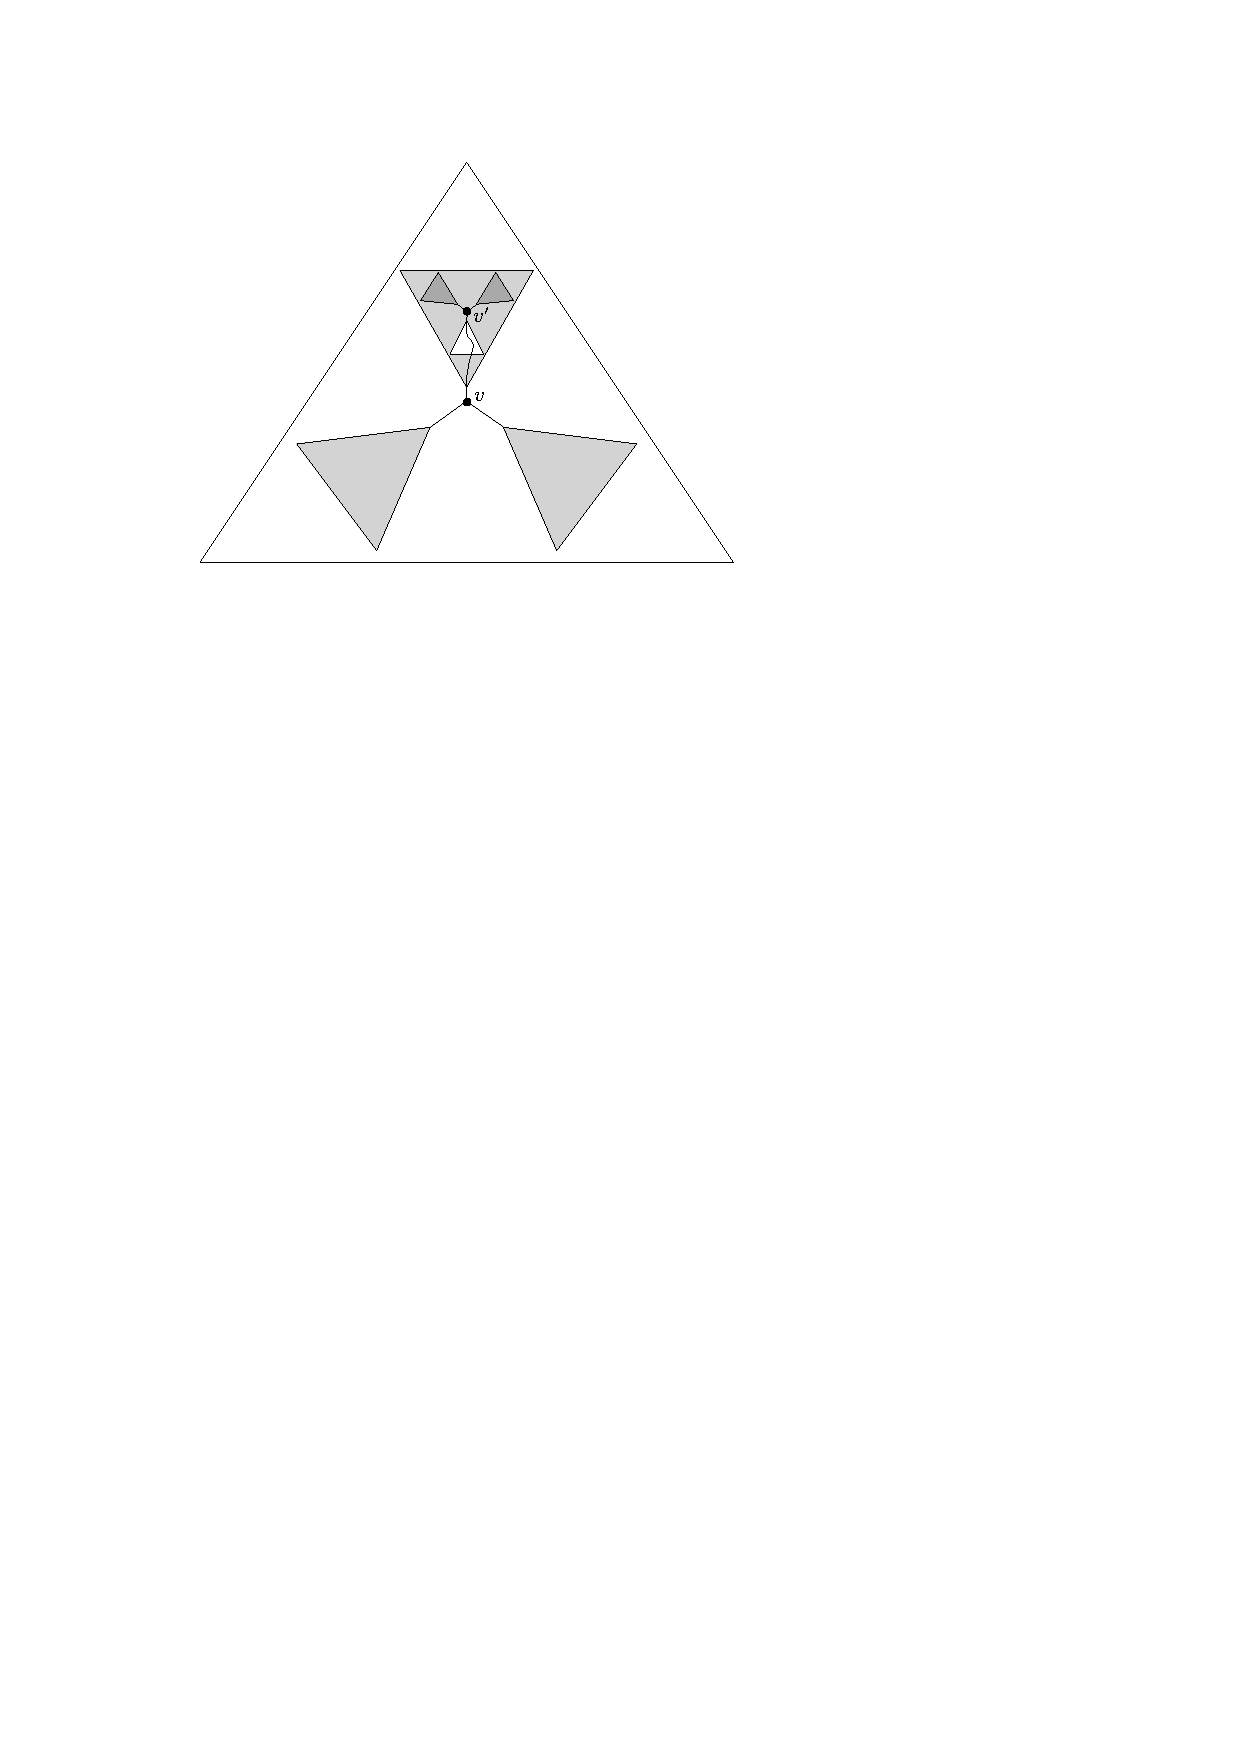
\includegraphics[scale=1]{centroid}
%\end{center}
%\caption{A single step in the centroid decomposition. Removing $v$ splits $T$ into three pieces, s.t. none of them has more than $\frac{|T|}{2}$ nodes. The white piece is problematic, since the paths from its nodes to $v$ do not pass through the inner centroid $v'$.}
%\end{figure}

To construct the matrices we apply the standard centroid decomposition. A node $v\in T$ is a centroid if every connected component of
$T\setminus\{v\}$ consists of at most $\frac{|T|}{2}$ nodes. The centroid decomposition of $T$ is defined recursively by first choosing a centroid
$v\in T$ and then recursing on every connected component of $T\setminus\{v\}$, which we call \emph{pieces}.
Overall, this process takes $O(b\log b)$ time. Since we assume that the input tree is binary, the centroid in every recursive call splits the tree
into three pieces. Now, we run the following bottom-up computation: assuming that we are given the three pieces, and for each of
them a sorted list of the distances to their centroid, we would like to compute a sorted list of distances of the nodes in all three pieces
to the centroid used to separate them. The difficulty is that we would like to produce this sorted list in linear time.

Consider one of the three already processed pieces obtained by removing the outer centroid. It contains three smaller pieces of its own,
that have been obtained by removing the inner centroid.
For two of these smaller pieces, it holds that the path from every node inside them to the outer centroid passes through the inner centroid.
We call the third piece, for which this does not hold, a \textit{problematic} piece. For the two pieces that are not problematic, we can 
increase all entries of their lists by the distance from the inner centroid to the outer centroid, and then merge two sorted lists in linear time.
Now consider the problematic piece, where paths to the outer centroid do not go through the inner one. Notice that if we go one step deeper
in the recursion, the problematic piece consists of two pieces that are not problematic, as the paths from all their nodes to the outer centroid
pass through their inner centroid, and the remaining even smaller problematic piece. For the two non-problematic pieces we can again
increase all entries of their lists and then merge two sorted lists in linear time, and repeat the reasoning on the problematic piece.
If the initial problematic piece was of size $s$, after $O(\log s)$ iterations we obtain that a sorted list of distances to the centroid can be
obtained by merging sorted lists of length $s,s/2,s/4,\ldots$, which can be done in $O(s)$ time. At every level of recursion, 
the total size of all the pieces is at most $b$, and there are $O(\log b)$ levels of recursion, so the total time spend on constructing
the sorted lists is $O(b\log b)$.

Finally, for every piece we define a row- and column-sorted matrix. If the sorted list of all distances of the nodes in the piece to the
centroid is $L[1..s]$, the entries of the matrix are $M[i,j]=L[i]+L[j]$. To represent $M$, we only have to store $L$, and then are able to
retrieve any $M[i,j]$ in $O(1)$ time. Note that some entries of $M$ do not represent distances between two nodes, but this is irrelevant.
To bound the number of matrices, observe that the total number of pieces is $b$, because after constructing a piece we remove the centroid.
To bound the total side length, observe that the side length of $M$ is bounded by the size of the corresponding piece, and the total size
of all pieces at the same level of recursion is at most $b$, so indeed the total side length is $O(b\log b)$.

\section{Full description of the linear algorithm for the dispersion optimization problem}\label{appendix linear algorithm for the dispersion optimization problem}

Consider a large fragment. It is composed of small fragments. Notice that some of these small fragments are active fragments, i.e. have not been reduced to caterpillars in the previous iteration, but most are inactive fragments, which have
been reduced to caterpillars. The large fragment contains some small fragments whose roots and holes are spine nodes of the large fragment,
and other fragments that form subtrees hanging off of the large fragment's spine (each hanging subtree may
contain several small fragments), see Figure \ref{figure of small fragments inside a large fragment}.

%\begin{figure}[h]
%\begin{center}
%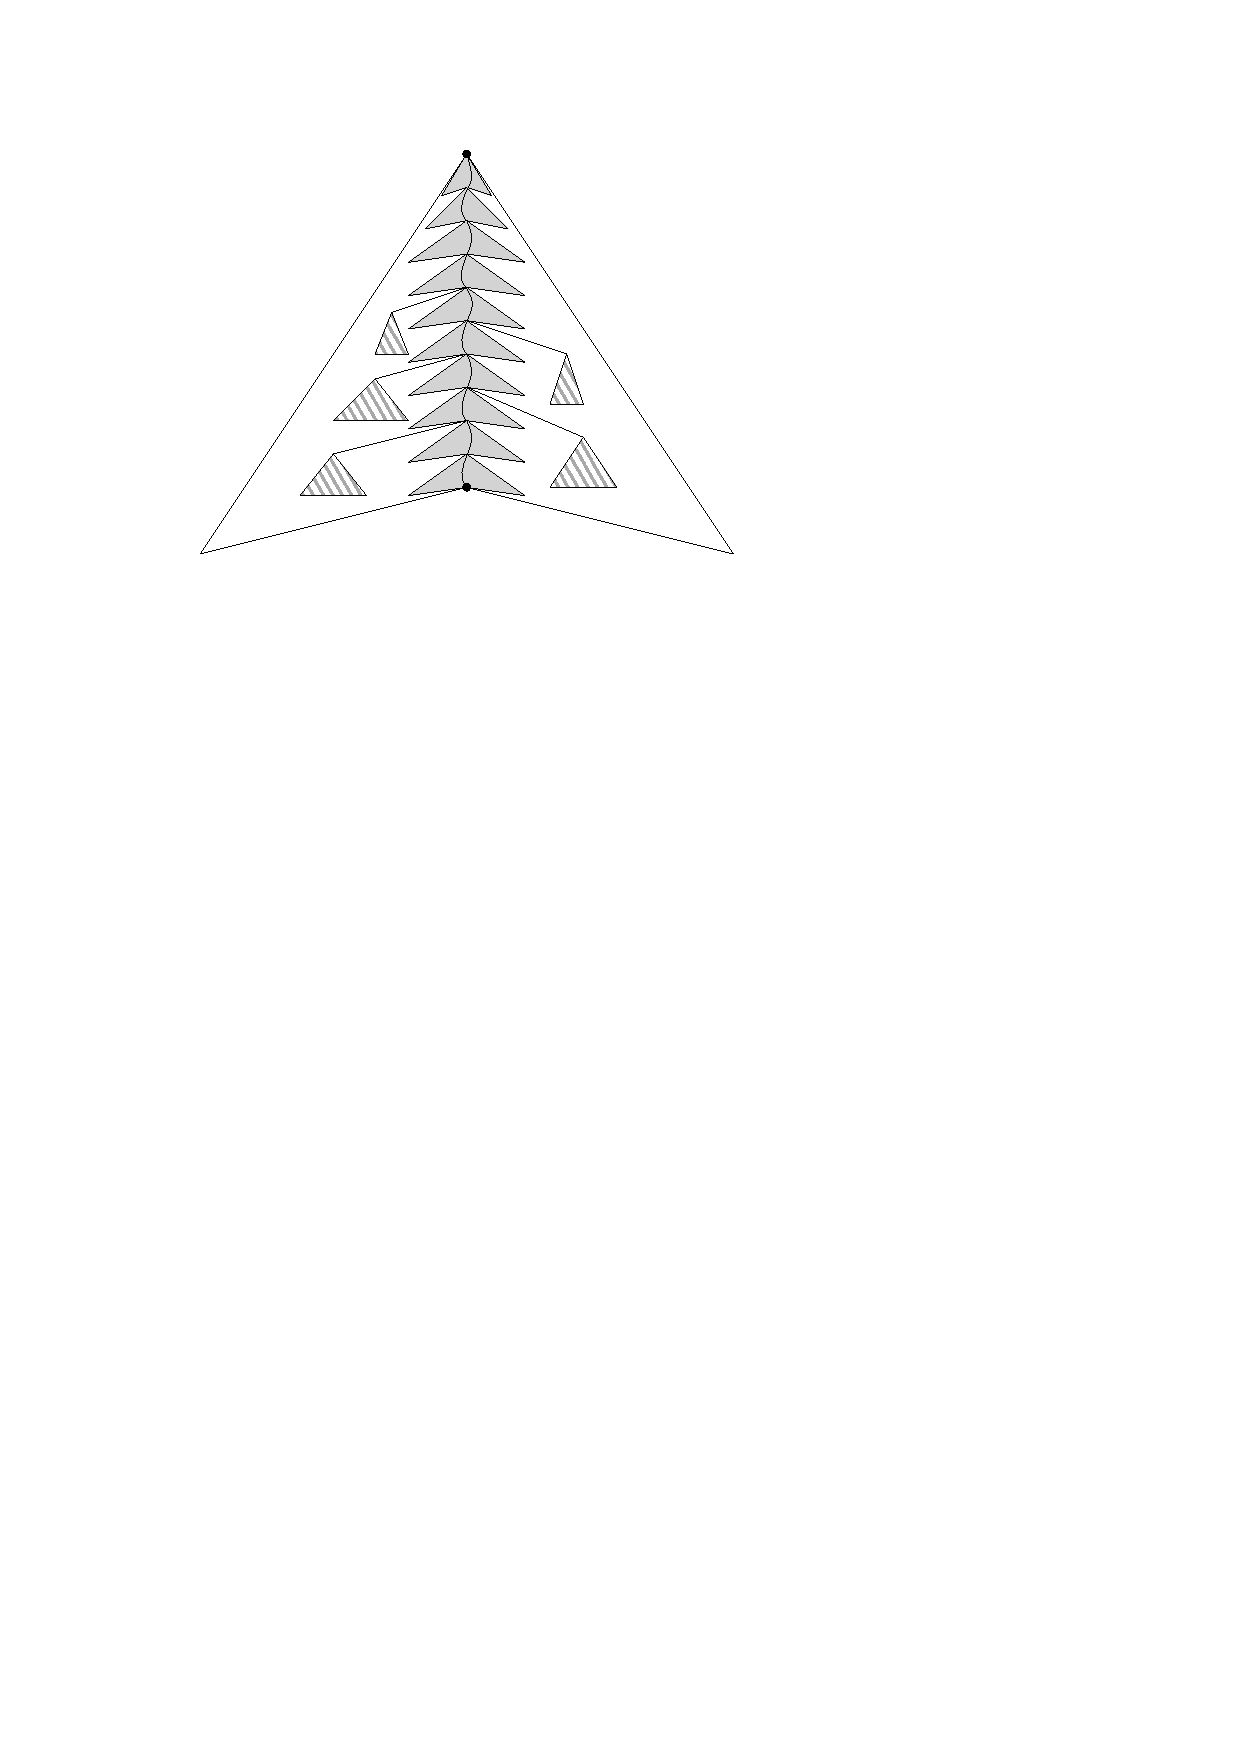
\includegraphics[scale=1]{refinement}
%\end{center}
%\caption{A large fragment containing a number of smaller fragments. The small fragments on the spine are gray, and the subtrees hanging off of the spine are black (each of them may contain many small fragments). %We start by reducing the hanging subtrees to just two nodes, then handle the small active fragments on the spine, and finally reduce the entire large fragment to one caterpillar and process it. 
%\label{figure of small fragments inside a large fragment}}
%\end{figure}


\noindent The partitioning used in the algorithm is presented in Subsection \ref{section:partioioning}. In Subsection~\ref{section:lemma1} we show how to reduce the hanging subtrees to at most two nodes, one candidate and one certain. Then, in Subsection~\ref{section:lemma2} we reduce the small active fragments on the spine to caterpillars. This turns the entire fragment into a large caterpillar. In Subsection~\ref{section:lemma3} we prune this large caterpillar so that it becomes monotone and without collisions. Finally, in Subsection~\ref{section:lemma4} we preprocess the resulting large caterpillar for eliminated suffix queries. 

\subsection{Partitioning into fragments}\label{section:partioioning}
We would like to partition the tree into fragments of growing sizes, and only spend linear time overall for this. We cannot repeatedly apply Lemma~\ref{basic partitioning lemma} as it is, since the constant hidden in its statement may become non-constant over the $\log^*n$ iterations. We therefore slightly augment the definition of a good partitioning, s.t. for a parameter $b$ it must have at most $n/b$ fragments, each of which is of size $O(b)$ (as opposed to the original definition, where we had $O(n/b)$ fragments of size at most $b$). We can achieve such a partitioning by applying Lemma \ref{basic partitioning lemma} with the parameter set to $b \cdot \alpha$, where $\alpha$ is the constant hidden in the statement of Lemma~\ref{basic partitioning lemma}. This results in a partition with at most $n/b$ fragments, each of size at most $\alpha \cdot b$. The following lemma uses this new definition.


\begin{lemma}\label{good partition refinement lemma}
Given a good partition of a binary tree into at most $n/b^{4}$ fragments each of size at most $\alpha^{\ell}\cdot b^{4}$, there
exists a good partition of the tree into at most $n/(2^b)^{4}$ fragments each of size at most $\alpha^{\ell+1}\cdot (2^{b})^{4}$,
where every fragment in the first partition is contained inside a fragment in the second partition.
\end{lemma}
\begin{proof}
Define $T'$ as the tree obtained by collapsing each fragment of the given partition into a single node. Partition $T'$ with the parameter set to $B= {(2^{b})^{4}}/{b^{4}}$. We obtain at most $\frac{n/b^4}{B}=n/(2^{b})^{4}$ fragments. Each of the new large fragments corresponds to a fragment of the original tree of size at most $\alpha\cdot \alpha^{\ell}\cdot b^{4}\cdot B = \alpha^{\ell+1}\cdot (2^{b})^{4}$. Clearly, it holds that each fragment of the given partition is contained in a single large fragment.
\end{proof}

\noindent The entire partition is obtained by applying Lemma~\ref{good partition refinement lemma} $\log^{*}n$ times. 
If $b_{\ell}$ denotes the value of the parameter $b$ in the $\ell$-th application, then  $b_{\ell+1}=2^{b_{\ell}}$. The time to construct the $(\ell+1)$-th partition is $O(n/(b_{\ell})^{4})=O(n/b_{\ell})$. The overall time to construct all partitions is therefore 
$$ O(\sum_{\ell} {n}/{b_{\ell}}) = O(\sum_{\ell} {n}/{2^{\ell}}) = O(n).$$
Observe that the size of a (large) fragment in the $(\ell+1)$-th partition is at most $\alpha^{\ell+1} \cdot (b_{\ell+1})^{4}$ which is at most $O((b_{\ell+1})^5)$ for a large enough $\ell$ (i.e., an $\ell$ s.t. $\alpha^{\ell+1}\leq 2^{2^{\ell+1}}$ and $b_{\ell+1}\geq 2^{2^{\ell+1}}$).  Denoting by $b=b_{\ell}$ and $B=b_{\ell+1}$  we get that every large fragment is of size $O(B^5)$ and is composed of (small) fragments of the $\ell$-th partition (each of size $O(b^5)$). 








\subsection{Reducing a hanging subtree into two nodes}\label{section:lemma1}
The first step in reducing a large fragment into a caterpillar is reducing the hanging subtrees of the large fragment into at most two nodes. The following lemma shows that this can be done in total $O(n)$ time for all fragments in all the $\log^* n$ partitions.




\begin{lemma}\label{lemma1}
	The hanging subtrees of the large fragments in all the partitions can be reduced to at most two nodes (one candidate and one certain) in total $O(n)$ time. 
\end{lemma}
\begin{proof}
We 
perform a heavy path decomposition on each hanging subtree. Since each such subtree is contained in a large fragment, its 
size is bounded by $O(B^5)$, and so we have at most $O(\log B)$ levels in the heavy 
path decompositions. On each level we run Frederickson's search (similarly to what we have presented before).
We run this search in parallel, for all heavy paths from all these hanging subtrees in all large fragments.
The number of  nodes in each level for all the heavy paths together is at most $m=n$ and we set
the parameter $p$ (in Theorem~\ref{Frederickson's theorem}) to $\frac{n}{B^{10}}$, so the number of calls to the $O(\frac{n}{b^4} \cdot \log b)$ time feasibility test
is $O(\max \lbrace \log(\max_{j} \lbrace n_j \rbrace), \log(\frac{m}{p+1}) \rbrace) = O(\max \lbrace \log (B^{5}), \log(\frac{n}{n/B^{10}} \rbrace) = O(\log B)$ per level, so
$O(\frac{n}{b^4} \cdot \log b \cdot \log^{2} B) = O(\frac{n}{b})$ for every iteration.
Summing over all $\log^{*}n$ iterations, this is $O(\sum_{\ell}\frac{n}{b_\ell}) = O(n)$.

Constructing the heavy path decompositions and then running Frederickson's search takes linear time in the number
of nodes in the subtrees. If all of them were then reduced to at most two nodes, one candidate and one certain
node for each subtree, this would take $O(n)$ time when summed over all the $\log^{*}n$  iterations. However, we have set
the parameter $p$ to $\frac{n}{B^{10}}$. Thus, considering all the levels, there
might be up to $\log B\cdot\frac{n}{B^{10}}\leq \frac{n}{B^{9}}$ large fragments in which we cannot fully reduce
all the hanging subtrees. These are active large fragments. We preprocess such fragments naively in time linear in their size. 
This requires only $O(\frac{n}{B^{4}})$ per iteration (and so $O(n)$ overall) since the total size of all active large fragments is at most
$\frac{n}{B^9} \cdot O(B^5)$. 
%We cannot amortize the time spent on processing their hanging
%subtrees  by simply saying that each such hanging subtree is reduced to at most
%two nodes, but we can easily afford to separately pay $O(\frac{n}{B^{4}})$ per iteration for this processing.
\end{proof}


\subsection{Reducing a small active fragment into a caterpillar}\label{section:lemma2}
Having processed the hanging subtrees, we now deal with the active small fragments on the spine of the large fragment. 

\begin{lemma}\label{lemma2}
	The small active fragments on the spines of all large fragments can be reduced to caterpillars in total $O(n)$ time. 
\end{lemma}
\begin{proof}

In the previous iteration we had $O(\frac{n}{b^9})$ active fragments, which is of course
too many for the current level. We take the remaining active small fragments (the ones on spines of large 
fragments), and reduce them to caterpillars (again by constructing the heavy path decomposition and running
Frederickson's search with $p$ set to $\frac{n}{B^{10}}$). In each fragment we have $O(\log b)$ levels of the heavy
path decomposition, and for each level we need $O(\log B)$ calls to the feasibility test, which takes
$O(\frac{n}{b^4} \cdot \log b \cdot \log B \cdot \log b) = O(\frac{n}{b})$ time in total. We also do linear
work exclusive of the feasibility tests. This processing of small active fragments takes $O(n)$ time over all
$\log ^*n$ iterations, by the same reasoning as for the hanging subtrees.
\end{proof}


We now have $O(\frac{n}{B^9})$ small active fragments in total. We declare each large fragment that contains a small active fragment as active. 

\subsection{Pruning the resulting large caterpillar}\label{section:lemma3}
So far, each inactive large fragment was reduced to one large caterpillar consisting of the concatenation of caterpillars from the smaller fragments on its spine. We want
to prune this large caterpillar (as we have done to the inactive fragments before) in order to ensure
that it is monotone and contains no collisions.   Then, we will
be able to preprocess the caterpillar for every possible eliminated suffix.

\begin{lemma}\label{lemma3}
	The inactive large fragments can be processed in overall $O(n)$ time so that each of them is a caterpillar, the distances of the leaves from the root and the hole are monotone, and there are no collisions between candidate nodes and certain nodes.
\end{lemma}
\begin{proof}

We start by pruning the large caterpillar so that distances of the candidates from the root are
monotone. Since the distances are monotone inside each small caterpillar, we only have to check the last (bottom most) 
candidate node of a small caterpillar against a range of consecutive candidates nodes below it in the large
caterpillar, starting from the top candidate node in the next small caterpillar. 
At this point we need to be more precise about how the fragments are represented. Each inactive small
fragment has been reduced to a caterpillar. For each such caterpillar, we maintain a doubly-linked list containing
all of its candidate nodes in the natural order, and additionally we store the first and the last certain
node (nearest to the root and to the hole, respectively). Assuming such representation, we traverse
the large caterpillar from bottom to top while
maintaining a stack with the already processed small caterpillars that still contain some candidate nodes.
We retrieve the last candidate of the current small caterpillar and eliminate the appropriate candidate
nodes below it. This is done by iteratively retrieving the top small caterpillar from the stack and then
accessing its top remaining candidate node $u$. If the distance of $u$ from the root is too small, we
remove $u$ from the front of its doubly-linked list, pop the list from the stack if it becomes empty,
and repeat. Now the distances of the remaining candidates from the root are
non-decreasing. We repeat the symmetric process from top to bottom to ensure that also the distances
from the hole are non-decreasing. The whole procedure takes linear time in the number of eliminated
candidate nodes plus the number of small fragments, which sums up to $O(n)$ overall.

Now we need to eliminate all internal ``collisions'' inside the large caterpillar (i.e. remove candidate nodes that
are too close to certain nodes). These collisions can occur between a candidate node of one small caterpillar
and a certain node of another small caterpillar. Each certain node eliminates a range of consecutive
candidates nodes below and above its small caterpillar. Therefore, we only need to consider the 
last certain node of a small caterpillar and a range of consecutive candidate nodes below it in the
large caterpillar, starting from the top candidate node in the next caterpillar (and then repeat
the reasoning for the first certain node and a range of candidates nodes above it). This seems very similar
to the previous step, but in fact is more complex: a certain node $v$ eliminates a candidate node $u$ when
$d(u,v)<\lambda^{*}$, but we do not know the exact value $\lambda^{*}$ yet! Therefore, we need to run
a feasibility test to determine if $u$ should be eliminated. We cannot afford to run many such tests
independently and hence will again resort to Frederickson's search. Before we proceed, observe that
it is enough to find, for every small caterpillar, the nearest certain node $v$ above it, and then determine
the prefix of the small caterpillar that is eliminated by $v$. To find $v$ for every small caterpillar,
we first traverse the large caterpillar from top to bottom while maintaining the nearest certain node
in the already seen prefix.

To apply Frederickson's search, we would like to create a matrix of dimension $1\times O(b^{5})$
for each of the $O(\frac{n}{b^{4}})$ small caterpillars in the whole tree. The total size of all small
caterpillars is at most $m=n$, so setting $p$ to $\frac{n}{B^9}$ would imply
$O(\max \lbrace \log(\max_{j} \lbrace n_j \rbrace), \log(\frac{m}{p+1}) \rbrace) = O(\max \lbrace \log (b^{5}), \log(\frac{n}{n/B^{9}} \rbrace) = O(\log B)$ calls to the $O(\frac{n}{b^{4}} \cdot \log b)$ time test.
There are two difficulties, though. First, we cannot guarantee that the processing exclusive of the feasibility tests
would sum up to $O(n)$ over all iterations. Second, it is not clear how to provide constant time access
to these matrices, as the candidates nodes inside every small caterpillar are stored in a doubly-linked list,
so we are not able to retrieve any of them in constant time. 
%We could have maintained the candidate
%nodes in an array, but then after the whole pruning and eliminating we would need to merge the arrays
%of all small caterpillars to obtain the array of the large caterpillar, which  does not seem possible
%in constant time (and we cannot afford to spend much more per a small caterpillar).

We mitigate both difficulties with the same trick. We proceed in $O(\log b)$ steps that, intuitively, correspond
to binary searching for how long should the eliminated prefix be. In the $i$-th step we
create a matrix of dimension $1\times 2^{i}$ for each of the still remaining small caterpillars.
The matrix is stored explicitly, that is we extract the top $2^{i}$ candidates nodes from the doubly-linked
list and store them in an array. We set $p$ to $\frac{n}{B^{10}}$ and run Frederickson's search
on these matrices. Then, if all $2^{i}$ candidate nodes have been eliminated, we proceed to the next
step. Otherwise we have already determined the small caterpillar's prefix that should be eliminated. The total time for all feasibility tests is then
$O(\frac{n}{b^{4}}\cdot \log b \cdot \log b \cdot \log B) = O(\frac{n}{b})$. 
Observe that the total length of all arrays constructed during this procedure is bounded by the number
of eliminated candidate nodes multiplied by 4. Consequently, both the time necessary
to extract the top candidate nodes (and arrange them in an array) and the time exclusive of the feasibility tests sums up to $O(n)$
over all iterations. During this process we might declare another $O(\frac{n}{B^9})$ large fragments active
by the choice of $p$.
\end{proof}


\subsection{Preprocessing the large caterpillar for every possible eliminated suffix}\label{section:lemma4}

Having reduced a large fragment to a large caterpillar, we are now left only with preprocessing this large caterpillar for every possible eliminated suffix.
Because we have already pruned the large caterpillar and removed any collisions between a certain
node and a candidate node, we only have to consider the remaining candidate nodes.
Recall that in the previous algorithm we stored at the bottom node of every prefix of the caterpillar
the following information: the number of chosen nodes, the candidate node, and the certain node for this fragment,
assuming that the suffix below this node is eliminated. Now however, we cannot afford to explicitly
compute such information for every node in every iteration,
as this might take linear time per iteration. We start with reinterpreting it in terms of
\emph{jump pointers}. 

\medskip \noindent {\bf Jump pointers.} For each candidate node in a caterpillar, its jump pointers leads to the nearest
candidate above (in the same caterpillar) that is at distance at least $\lambda^{*}$. Then, the information
stored at the bottom node $u$ of every prefix can be computed by starting at $u$ and following
the jump pointers as long as possible. The number of nodes chosen for the solution is simply the number of visited
nodes. If the last visited node is at distance at least $\frac{\lambda^{*}}{2}$ from the root then it is
the certain node, and otherwise the last visited node is the candidate node and its predecessor
(if any) is the certain node. We would like to maintain such information for all nodes $u$,
such that $u$ might be accessed in query time. Recall that in query time we specify
a node $v$ attached to the hole of the fragment and binary search for the first node $u$ that
is at distance at least $\lambda^{*}$ from $v$. Therefore, we only need to maintain the information
for a suffix consisting of nodes that are not too far from the hole (i.e. at distance at most $\lambda^{*}$). However, it is not
 trivial to update such information after merging multiple small caterpillars into
one. This is because we might remove some nodes (a prefix and a suffix)
from every small caterpillar before the merge. To overcome this, we divide every caterpillar into
three parts as described below.

\medskip \noindent {\bf The unstable prefix,  unstable  suffix, and stable infix.} 


Consider a caterpillar with root $r$ and hole $h$, and let $u_{i}$ denote its $i$-th candidate node. In Lemma~\ref{lemma3} we have already made sure that $d(r,u_{i}) < d(r,u_{i+1})$
and that $d(h,u_{i}) > d(h,u_{i+1})$. We define the \emph{unstable prefix} to
consist of all nodes $u_{i}$ such that $d(r,u_{i})\leq \frac{\lambda^{*}}{2}$, and similarly the
\emph{unstable suffix} consists of all nodes $u_{i}$ such that $d(h,u_{i})\leq \frac{\lambda^{*}}{2}$.
The remaining nodes $u_{i}$ are called the \emph{stable infix}.  We have the following property.

\begin{lemma}
\label{stable infix}
If a node of a small caterpillar is removed due to the pruning or collision elimination then it
belongs to the unstable prefix or to the unstable suffix.
\end{lemma}

\begin{proof}
Because of symmetry, it is enough to consider a small caterpillar and all the subsequent
small caterpillars. If a candidate node $u_{i}$ of the former is pruned then there is a top candidate node
$v$ of one of the subsequent caterpillars such that $d(h,u_{i}) < d(h,v)$, where $h$ is the hole
of the large caterpillar. But the distance of $v$ from the spine is less than $\frac{\lambda^{*}}{2}$ (since it is a candidate node),
 and it follows that the distance of $u_{i}$ to the hole of its small caterpillar is also less
than $\frac{\lambda^{*}}{2}$. If $u_{i}$ collides with a certain node $v$ of one of the subsequent
caterpillars then $d(u_{i},v)<\lambda^{*}$. But the distance of $v$ from the spine is at least
$\frac{\lambda^{*}}{2}$, so the distance of $u_{i}$ to the hole of its small caterpillar must be
less than $\frac{\lambda^{*}}{2}$. Hence, $u_{i}$ belongs to the unstable suffix.
\end{proof}

We maintain the unstable prefix and the unstable suffix  in balanced search
trees (sorted by the distance to the root or the hole) that allow split and join in logarithmic time.
The stable infix is maintained in a separate structure that allows us to efficiently simulate traversing jump pointers inside the stable infix. 
%
In query time, we first use the balanced search tree storing the unstable suffix to locate the bottom-most node
$u_{i}$ that is sufficiently far away. Observe that after taking $u_{i}$ we cannot
take any further nodes from the unstable suffix, as they are all within distance less than
$\lambda^{*}$ from each other. Hence, we need to continue in the stable infix (it can also
happen than no $u_{i}$ from the unstable suffix can be taken, and we directly start in the stable
infix). Then, we use the structure maintained for the stable infix, which gives us the top-most
node that we would reach by following up the jump pointers. Finally, we  continue in the unstable prefix. 

By the same argument as before, we can visit at most one node in the unstable prefix.
Therefore, if we can efficiently answer a query in the stable infix, then answering a query in
the whole caterpillar requires only additional logarithmic time (in the size of the caterpillar).
Additionally, after merging multiple small caterpillars into one, we need to determine the unstable
prefix and the unstable suffix of the resulting large caterpillar and make sure that we have
their corresponding binary search trees available.
Then we have to construct the structure for the stable infix of the large caterpillar.
We next describe these two steps.

\medskip \noindent {\bf Maintaining the unstable suffixes.}
Consider the unstable suffix of the large caterpillar (the situation for the unstable prefix is
symmetric). It is easy to see that all of its nodes are contained in unstable suffixes of
the small caterpillars. We merge all the binary search trees storing these unstable suffixes.
This takes $O(\log (B^5))$ time per merge, so $O(\frac{n}{b^{4}}\cdot \log (B^5))=O(\frac{n}{b})$ in total.
Then, we binary search to determine how many nodes are actually sufficiently close to the hole of the large caterpillar, and
 split the binary search tree accordingly in $O(\log (B^{5}))$ time. To implement binary search, we need to
check if a distance from a node to the hole is at least $\frac{\lambda^{*}}{2}$, but of course we
do not know $\lambda^{*}$ yet. Therefore, we perform all these binary searches in parallel. We proceed in $O(\log (B^{5}))$ rounds. In every round we apply Frederickson's search
with parameter $p$ set to $\frac{n}{B^{10}}$ to determine  the outcome of the comparison for all
but $\frac{n}{B^{10}}$ binary searches. This needs
$O(\frac{n}{b^{4}}\cdot\log b\cdot\log B\cdot\log B)=O(\frac{n}{b})$ additional time for
all the feasibility tests and creates additional $O(\frac{n}{B^{9}})$ active large fragments.

\medskip \noindent {\bf Maintaining the stable infixes.}
We now describe the structure for maintaining the stable infix of a caterpillar consisting of candidate nodes $u_{1},u_{2},\ldots,u_{k}$ with root $r$ and hole $h$. 
Recall that, for each candidate node $u_i$, its jump pointer leads to the closest candidate node above it (in the same caterpillar) that is at distance at least $\lambda ^*$. 
We need a structure that allows us to query, given a node $u$ attached to $h$, for the nearest candidate node $u_{i}$ at distance at least $\lambda^{*}$ from $u$, and then follow the jump pointers from $u_{i}$.
%
Observe that we only consider $u$ such that $d(r,u)\geq d(r,u_{k})$. This is because either $u$ is a certain node and then its distance from the hole is at least
$\frac{\lambda^{*}}{2}$, or $u$ is a subsequent candidate node from the same caterpillar,
or we start the query with comparing these two distances.

We are interested in the number of traversed jump pointers and in the last visited node.
%(because of the unstable prefix, we do not need to retrieve both the last node
%and its predecessor). 
During the preprocessing, we need to merge multiple stable infixes
into one, while possibly inserting some nodes in-between (these new nodes have previously
belonged to some unstable prefixes and suffixes). To find $u_{i}$, we keep all candidate
nodes of a caterpillar in a mergeable balanced search tree. This allows us to locate $u_{i}$
in logarithmic time (in the size of the caterpillar), and the total time to construct the balanced
search trees for all stable infixes by merging the smaller balanced search trees
is $O(\frac{n}{b^{4}}\cdot \log (B^{5}))=O(\frac{n}{b})$. Note that the smaller balanced search
trees could either be associated with a stable infix of a small caterpillar or be obtained
by splitting a balanced search tree stored for an unstable prefix or an unstable suffix of
a small caterpillar.
We will show how to maintain the answer, that is the number of traversed jump pointers and the
last visited node, explicitly for every $u_{i}$ that could be queried.

We write $\jump(i)=j$ if the jump pointer of $u_{i}$ points to $u_{j}$, where $j<i$, and $\jump(i)=-1$
if the jump pointer of $u_{i}$ is not defined, that is $d(u_{1},u_{i})<\lambda^{*}$.
The {\em interesting prefix} of the caterpillar consists of all nodes $u_{i}$ such that $\jump(i)=-1$,
and the {\em interesting suffix} consists of the nodes $u_{\jump(k)},u_{\jump(k+1)},\ldots,u_{k}$.
Because we always query with a node $u$ such that $d(r,u) \geq d(r,u_{k})$, we only
need to maintain the answer for the nodes in the interesting suffix. As a special case,
if $\jump(k)=-1$ we call the caterpillar \emph{fresh}.
After merging multiple small caterpillars into one we might need to update some of the jump pointers.
However, once a jump pointer has been set, it will never change. Therefore, we might only
need to set up the jump pointers in the interesting prefixes of the small caterpillars
(and the new nodes inserted in-between). We also observe that these new jump pointers
must lead either to a node in the interesting suffix of some small caterpillar
or to some new node. We start with checking if the large caterpillar is fresh. This can be
done by applying Frederickson's search in parallel for all large caterpillars with $p$ set to
be $\frac{n}{B^{9}}$, using $O(\frac{n}{b^{4}}\cdot \log b \cdot \log B)=O(\frac{n}{b})$
total time for the feasibility tests and creating up to $O(\frac{n}{B^{9}})$ additional active large
fragments. If a large caterpillar is fresh, there is nothing to update. Otherwise,
we gather all candidate nodes belonging to
an interesting prefix or suffix (or being a new node) and call them \emph{relevant}. In particular,
all nodes of a fresh small caterpillar are relevant.
We arrange all relevant nodes in an array and apply Frederickson's search to determine the missing jump
pointers using the array to facilitate constant time access to any relevant node. We again
set $p$ to be $\frac{n}{B^{9}}$, need $O(\frac{n}{b^{4}}\cdot \log b \cdot \log B)=O(\frac{n}{b})$
time for the feasibility tests, and create $O(\frac{n}{B^{9}})$ additional active large fragments.
The time exclusive of the feasibility tests is bounded by the number of relevant nodes.
We claim that once we know all the missing jump pointers we can actually update the answers
for all nodes in the interesting suffix of the large caterpillar in time proportional to the
number of relevant nodes. This is because all nodes of that interesting suffix are
relevant, and we can update the answer for all relevant nodes by traversing them from top
to bottom. The current candidate node either already had a jump pointer before, and hence
we can use its previously computed answer to access an already processed relevant node
(as all nodes in an interesting prefix are relevant, and the answer is always a node in an
interesting prefix by definition) and, by combining with the already updated answer for that
relevant node, recalculate the answer, or follow its freshly found jump pointer to also access
an already processed relevant node. The total time for this update is again proportional to the
number of relevant nodes. It remains to bound this quantity. We claim that it
amortizes to $O(n)$. To this end, we maintain the following invariant: every node
of an interesting prefix and suffix has one credit. If a caterpillar is fresh
then every node $u_{1},u_{2},\ldots,u_{k}$ has two credits. Initially, every node of the tree
has two credits. When a node becomes a part of a stable infix we treat it as a small fresh
caterpillar in the analysis. The number of relevant nodes is bounded by the total number
of nodes in all fresh small caterpillars and the total number of nodes in the interesting
prefixes and suffixes in the remaining small caterpillars. Furthermore,
the interesting prefix (and similarly the interesting suffix) of the resulting large caterpillar
consists of nodes belonging to fresh small caterpillars and the interesting prefix of
some small caterpillar. So to pay for all relevant nodes and then make sure that the invariant
still holds we only need additional $O(b^{5})$ credits (to pay for the interesting prefix
of some small caterpillar and the interesting suffix of some small caterpillar) per large
caterpillar. This sums up to $O(\frac{n}{B^{4}}\cdot b^{5}) = O(\frac{n}{b})$ per iteration.

To conclude, we have shown how to obtain an $O(\frac{n}{B^{4}}\log B)$ time test given an $O(\frac{n}{b^{4}}\log b)$
time test, in $O(\frac{n}{b})$ time plus amortized constant time per
node. After $\log ^*n$ iterations, we have a $O(\frac{n}{\log ^4n} \cdot \log \log n)$ test,
which we use to solve the dispersion optimization problem in linear time. All iterations of the preprocessing
cost $O(n)$ time altogether.
% why do we stop at fragments of size polylog(n)? Can't we get one large fragment?

\section{An \texorpdfstring{\boldmath$ \Omega (n\log n)$}{Omega(nlogn)} lower bound for the weighted feasibility test}\label{appendix weighted f.t. lower bound}

In the {\em Set Disjointness} problem, we are given two sets of real numbers $X=\lbrace x_1,x_2,\ldots,x_n \rbrace$ and $Y=\lbrace y_1,y_2,\ldots,y_n \rbrace$ and we need to return true iff $X \cap Y = \emptyset$. 
It is known that solving the set disjointness problem requires $\Omega(n \log n)$ operations in the algebraic
computation tree model~\cite{BenOr}.
We present a reduction from the set disjointness problem to the weighted feasibility test problem. We assume without loss of generality that the elements of $X$ and $Y$ are non-negative (otherwise,
we find the minimum element and subtract it from all elements).


Given the two sets $X$ and $Y$, we construct a tree $T$ as follows. We first compute and set
$K := 2 \cdot \max (X\cup Y) +3$.
The tree $T$ contains two vertices of weight zero, $u$ and $v$, that are connected by an edge of length $\frac{K}{2}$. In addition, for each element $x_i \in X$, we have a node of weight $x_i+1$, that is connected to $u$ by an edge of length $\frac{K}{2} - x_i -1$. For each element $y_i \in Y$, we have a node of weight $K - y_i -1$, that is connected to $v$ by an edge of length $y_i+1$.
\begin{lemma}\label{lemma of the reduction to set disjointness}
$X \cap Y = \emptyset$ iff the weighted feasibility test returns false for $T$ with  parameters $W=K$ and $\lambda =K$.
\end{lemma}

\begin{proof}
We start by proving that if $X \cap Y \neq \emptyset$ then there is a subset of the vertices of the tree, $P \subseteq T$, s.t. $W(P) \geq K$ and $f(P) \geq K$ (where $W(P)$ is the sum of the weights of all the vertices in $P$). Suppose that  $x_i=y_j$. Then, $d(x_i,y_j) = d(x_i,u) + d(u,v) + d(v,y_j) = \frac{K}{2} - x_i -1 + \frac{K}{2} + y_j +1 = K \geq K$. Furthermore, $W(x_i) + W(y_j) = x_i + 1 + K- y_j -1 = K \geq K$, and so the feasibility test should return true due to $P = \lbrace x_i, y_j \rbrace$.

Now we need to prove that if the feasibility test returns true, the sets are not disjoint.
We start by proving that any feasible subset $P$ cannot have more than one vertex from each of the sets.
Assume for contradiction that $P'$ is a feasible subset that contains at least two vertices that correspond to elements of $X$. Denote these two vertices by $x_i$ and $x_j$. We assume that $P'$ is a feasible solution, and so $d(x_i,x_j) \geq K$. But, $d(x_i,x_j) = \frac{K}{2} - x_i -1 + \frac{K}{2} - x_j -1 = K - x_i - x_j -2 < K$ (since $x_i$ and $x_j$ are non-negative) and we have a contradiction.
If $P'$ contains two elements of $Y$, denoted $y_{i}$ and $y_{j}$, we also obtain a contradiction because
$d(y_{i},y_{j})=y_{i}+1+y_{j}+1<K$.
Observe that it is also not possible for $P$ to contain only one node, since the weight of any node is strictly less than $K$. So, we now only need to prove that if $P= \{ x_i,y_j \}$ is a feasible solution, then $x_i = y_j$.
If $P= \{ x_i,y_j \}$ is a feasible solution then on the one hand $d(x_i,y_j) = \frac{K}{2} - x_i -1 + \frac{K}{2} + y_j +1 = K - x_i + y_j \geq K$, implying that $y_j \geq x_i$. On the other hand, $W(P) = x_i + 1 + K - y_j -1 = K + x_i - y_j \geq K$, implying that $x_i \geq y_j$. We conclude that $x_i = y_j$.
\end{proof}

\section{Batched operations}\label{appendix batched operations}
\subsection{Operation~\ref{op6} -- batched value predecessor}
Similarly to Operation~\ref{op5}, we start by describing a procedure that works on one tree, then apply the same trick of splitting the tree into small trees, and work on them.

We start each value predecessor query by first finding $k_i$ (or its predecessor, if there is no breakpoint at $k_i$). Then, we go up the path in the tree until the maximum value of a leaf in a subtree hanging to the left of the path is at least $v_i$. We then keep going down to the rightmost child that has at least $v_i$ as the maximum value in its subtree. The overall runtime is $O(x \log y)$ since each value predecessor query takes $O(\log y)$ time.

We now apply the same splitting procedure as in Operation \ref{op5}, and obtain $O(x)$ trees with $O(\frac{y}{x})$ leaves each. We would like to iterate over the given keys and run value predecessor queries. However, unlike in Operation \ref{op5}, now the intervals defined by the pairs $(k_i',k_i)$ are not necessarily disjoint and so we need to be more careful as to not spend more than constant time for each root of a small tree when we scan the roots.

Recall that we had two uses for the batched value predecessor operation. The first was to prune the non-monotone polyline we have obtained by increasing intervals of $p_2$ (see Figure~\ref{figure of the second case in the construction of the first half of the polyline}). The pruning is done by deleting the intervals returned by this operation.
%
Consider two consecutive keys $k_1$ and $k_2$ ($k_1 \leq k_2$) for which we would like to find their value predecessors $k_1'$ and $k_2'$. If the value of the polyline at $k_1$  is greater or equal to the value  of the polyline at $k_2$, then certainly $k_1 \leq k_2'$, and the intervals are in fact disjoint. Else, the intervals might not be disjoint, but we know that $k_1' \geq k_2'$, and so the interval $(k_1',k_1)$ is contained in the interval $(k_2',k_2)$. Thus, deleting the second interval is enough, meaning that we do not need to run the value predecessor query for $k_1$ at all. Generalizing this observation, before running the value predecessor queries, we can remove keys from the input list
so that the values of the remaining keys are  monotonically decreasing, in $O(x)$ time\footnote{In this case the values of the polyline at $k_1$ and $k_2$ are in fact $v_1$ and $v_2$ which are given as input, so we don't have to query for them. These values are obtained during the interval increases which precede this pruning of the non-monotone polyline.}. 
% by scanning them from left to right while maintaining the remaining keys on a stack.
We can then answer value predecessor queries for this pruned list of keys using our small trees with $O(\frac{y}{x})$ leaves. We process the keys from right to left while simultaneously scanning the small trees (also from right to left). To process a pair $(k_{i},v_{i})$ we first find $k_{i}$, then we continue moving to the previous small tree as long as the maximal value stored at the root is smaller than $v_{i}$. Once we find the appropriate small subtree, we run a value predecessor query on it (similarly to what we described for one tree). 
%
Therefore, we search for the value predecessor of each key in one small tree in $O(\log(\frac{y}{x}))$ time,
and additionally sweep through $O(x)$ roots, so the cost is $O(x \log (\frac{2y}{x}))$. We finish by merging the small trees back into one large tree (as in Operation \ref{op5}) which also takes $O(x \log (\frac{2y}{x}))$ time, and so this is also the time complexity of the entire operation.

The second use of this operation was to find the intersection points of two polylines. In this case it is easy to see that the intervals $(k_i',k_i)$ are in fact disjoint, since we query with the keys of the breakpoints of one of the polylines only when there must be an intersection point between this breakpoint and the previous one, and so we do not need any pruning.


\subsection{\bf Operation~\ref{op7} -- batched interval insertions.}
Again, we split the tree into small trees with $O(\frac{y}{x})$ leaves. Additionally, we split the small trees s.t. every interval
that should be inserted falls between two small trees.
Since we have at most $x$ such extra splits, each of which takes $O(\log(\frac{y}{x}))$ time, the total time for this is $O(x\log(\frac{2y}{x}))$.
Then, for every such breakpoint we create a small tree containing just a single leaf corresponding to that
breakpoint. Therefore, we have $O(x)$ small trees with $O(\frac{y}{x})$ leaves that should be now merged
to obtain one large tree.
The merging is done as in the previous operations, and the total cost can be bounded,
up to a constant factor, by essentially the same calculation as in Lemma \ref{running time to obtain small trees lemma}. Therefore, the overall time for the operation is $O(x \log(\frac{2y}{x}))$.

\subsection{\bf Operation~\ref{op8} -- batched interval deletions.}
Once again we split our tree into small trees. We then delete the relevant intervals from each of the small trees. Each interval is either contained in a single small tree (and is then deleted by performing one or two split operations and at most one join operation) or it spans several small trees (in which case we might also need to delete some trees entirely). This takes $O(x \log(\frac{2y}{x}))$ time in total.

\section{Figures}

\begin{figure}[ht]
{\caption{A fragment in a good partition consists of the subtree of $u$ without the subtree of $v$.
$u$ is the root, $v$ is the hole, and the path from $u$ to $v$ is the spine of the fragment.}}
{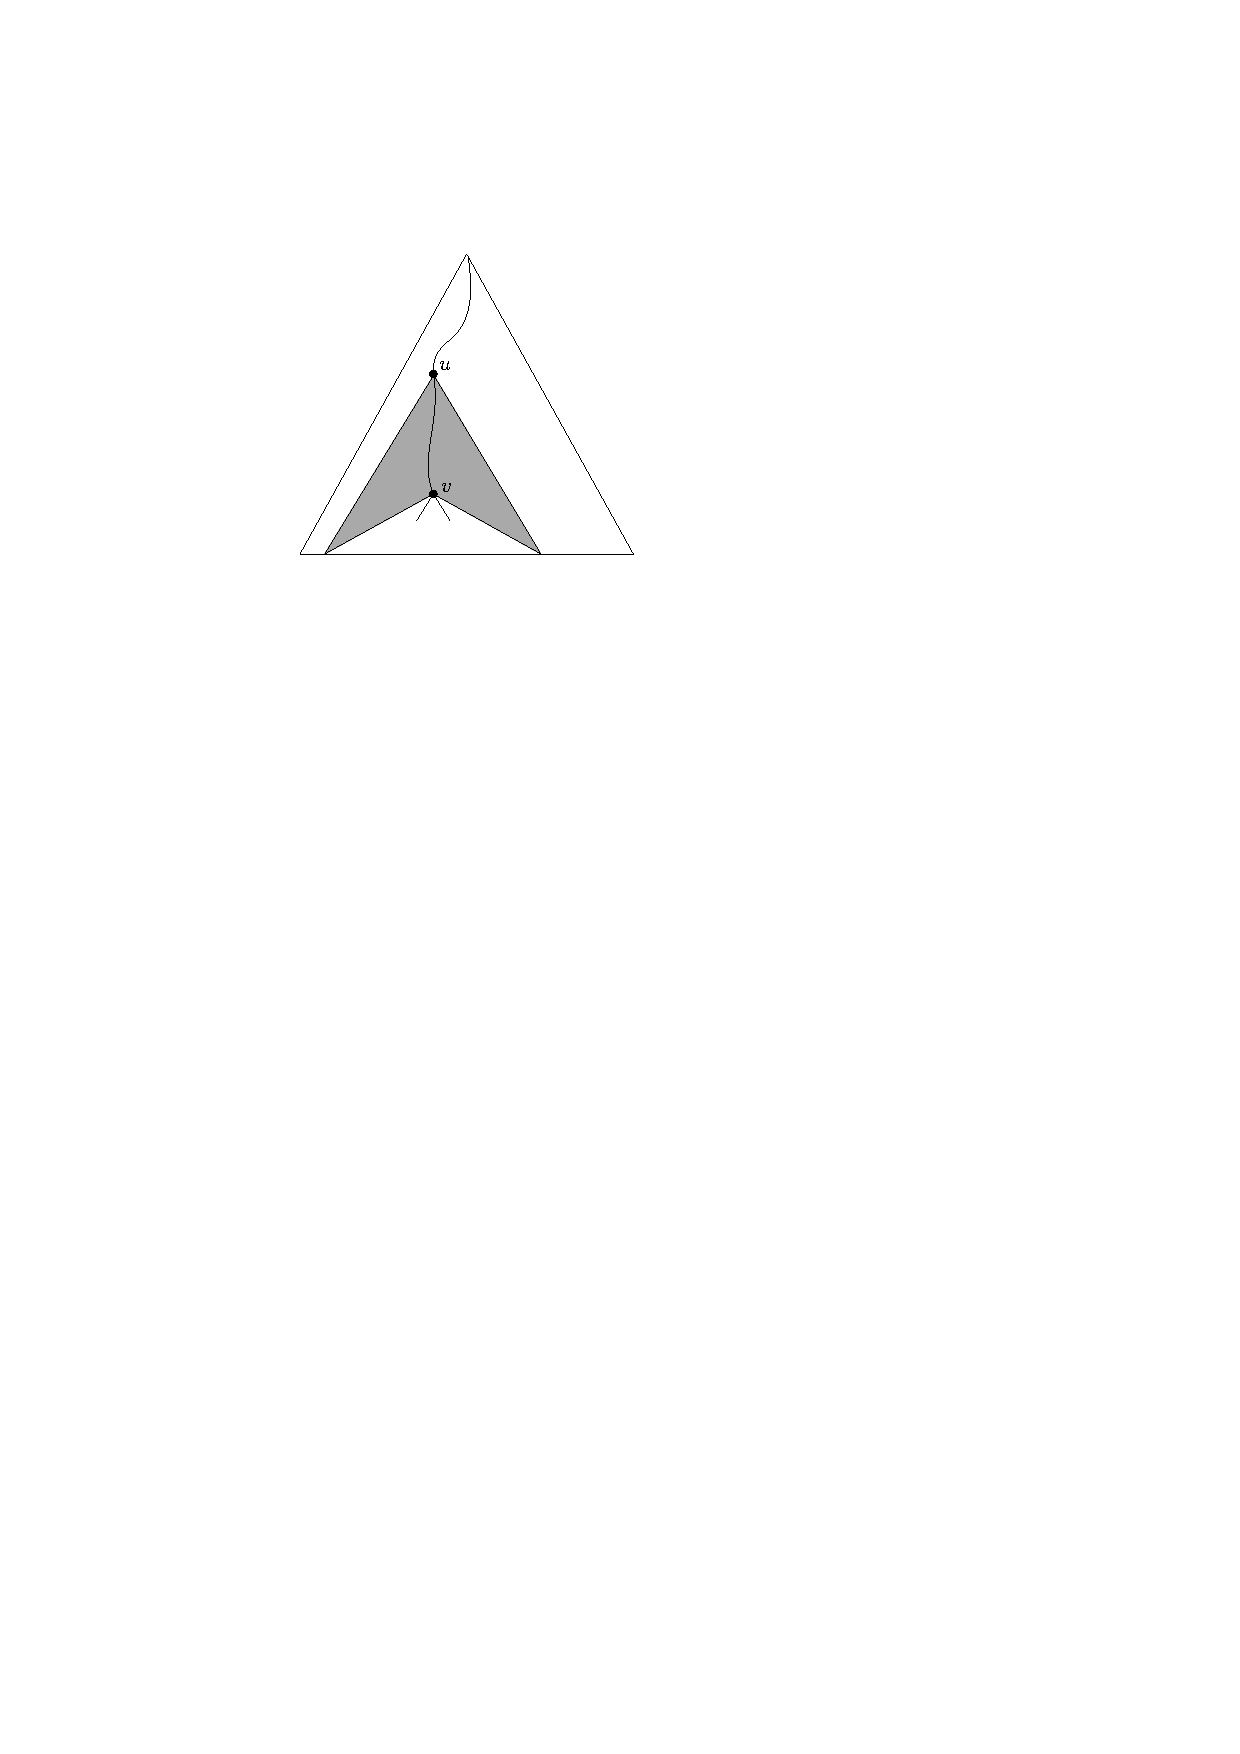
\includegraphics[scale=0.7]{fragment}}
\end{figure}

\begin{figure}[ht]
\begin{center}
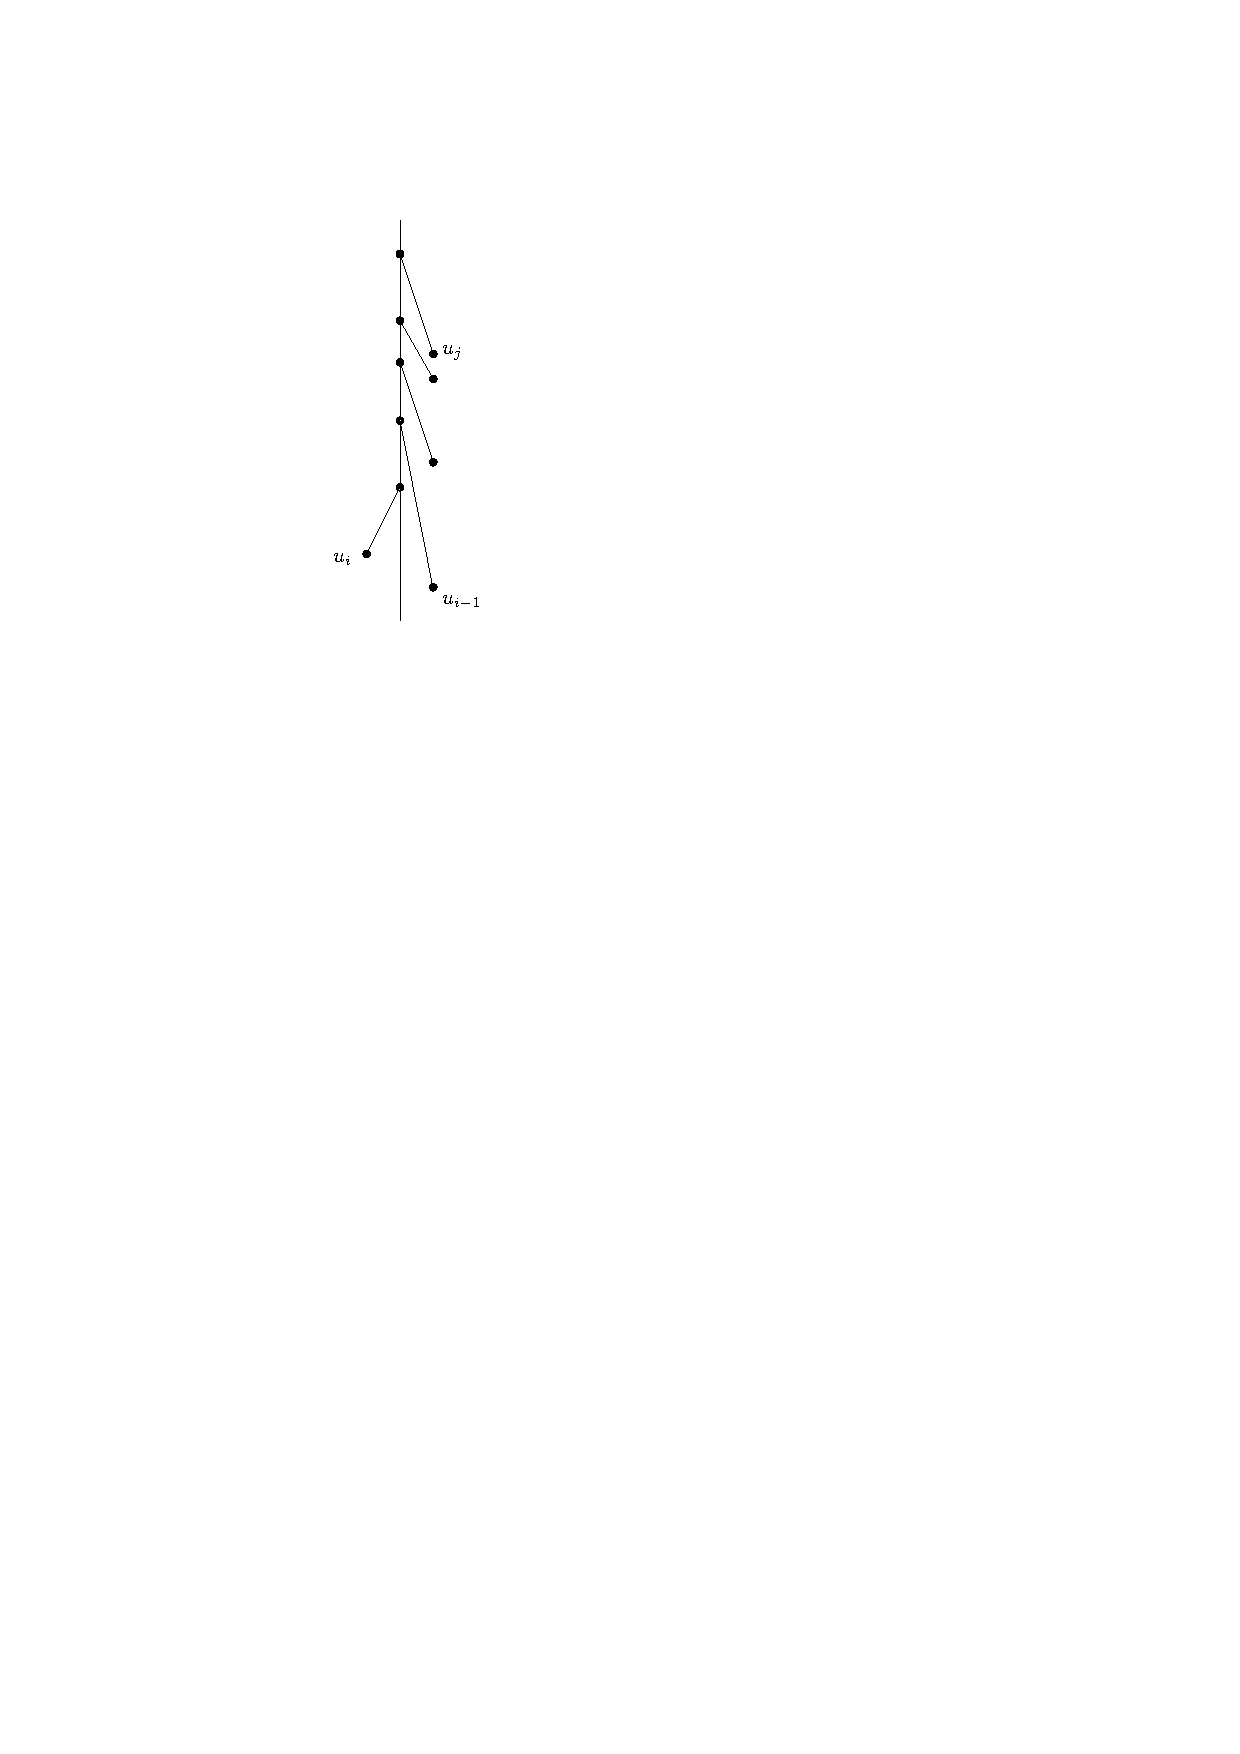
\includegraphics[scale=0.45]{caterpillar}
\end{center}
\caption{If $d(u_i,r)<d(u_{i-1},r)$ then  we can remove $u_{i}$ since (1) an optimal solution cannot contain both $u_{i}$ and $u_{i-1}$ (the distance between them is too small), and (2) if an optimal solution contains $u_{i}$ then it can be replaced with $u_{i-1}$ (every leaf $u_j$ is farther from $u_{i-1}$ than from $u_i$). \label{fig:pruning}}
\end{figure}

\begin{figure}[ht]
\begin{center}
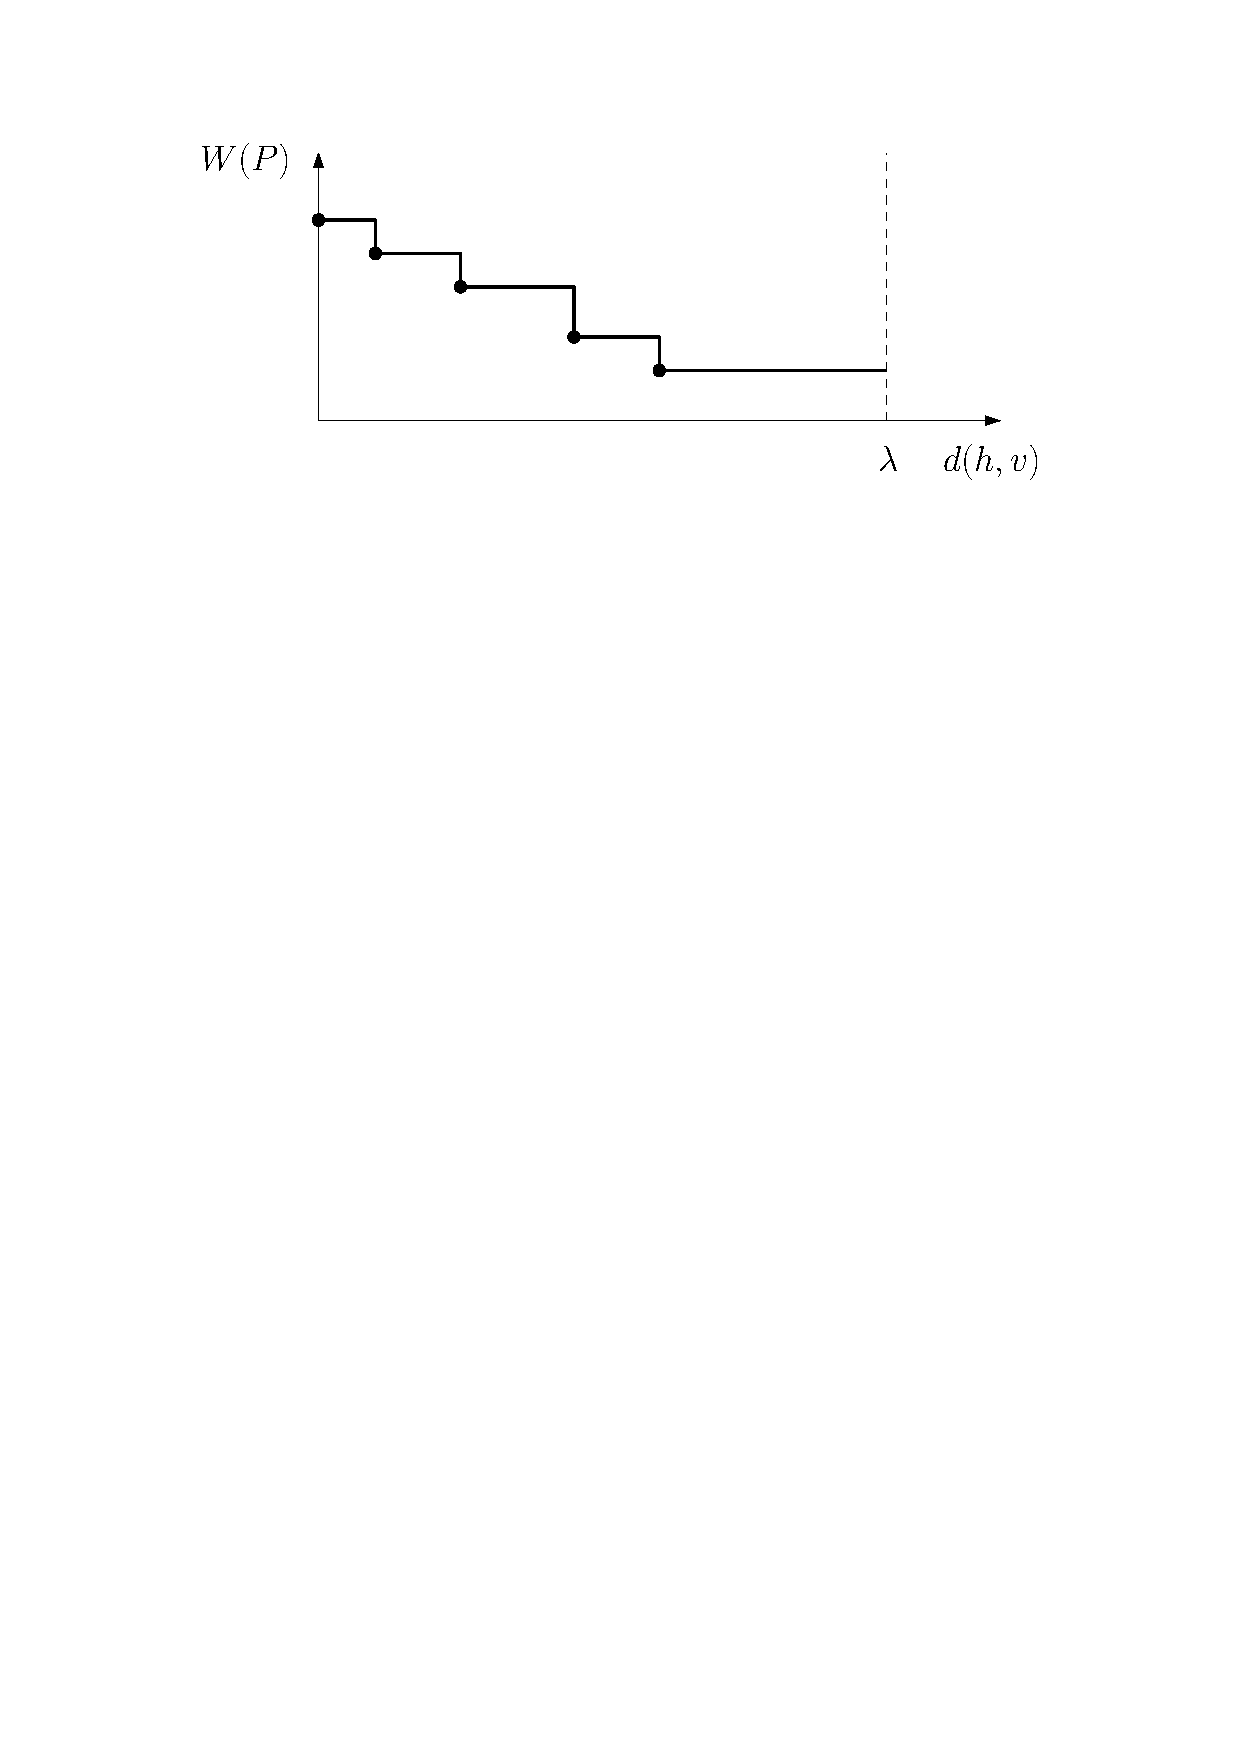
\includegraphics[scale=0.55]{polyline}
\end{center}
\caption{The polyline represents the weight of the optimal solution $P$ as a function of the distance of the closest chosen node in the subtree. %$v$ is the root of the subtree, and $h$ is the chosen node closest to $v$ in its subtree. 
The weight of $P$ only decreases at certain points called breakpoints (in bold). Each breakpoint stores the value in the interval between itself and the next breakpoint.
\label{figure of a polyline}}
\end{figure}


\begin{figure}[ht]
\begin{center}
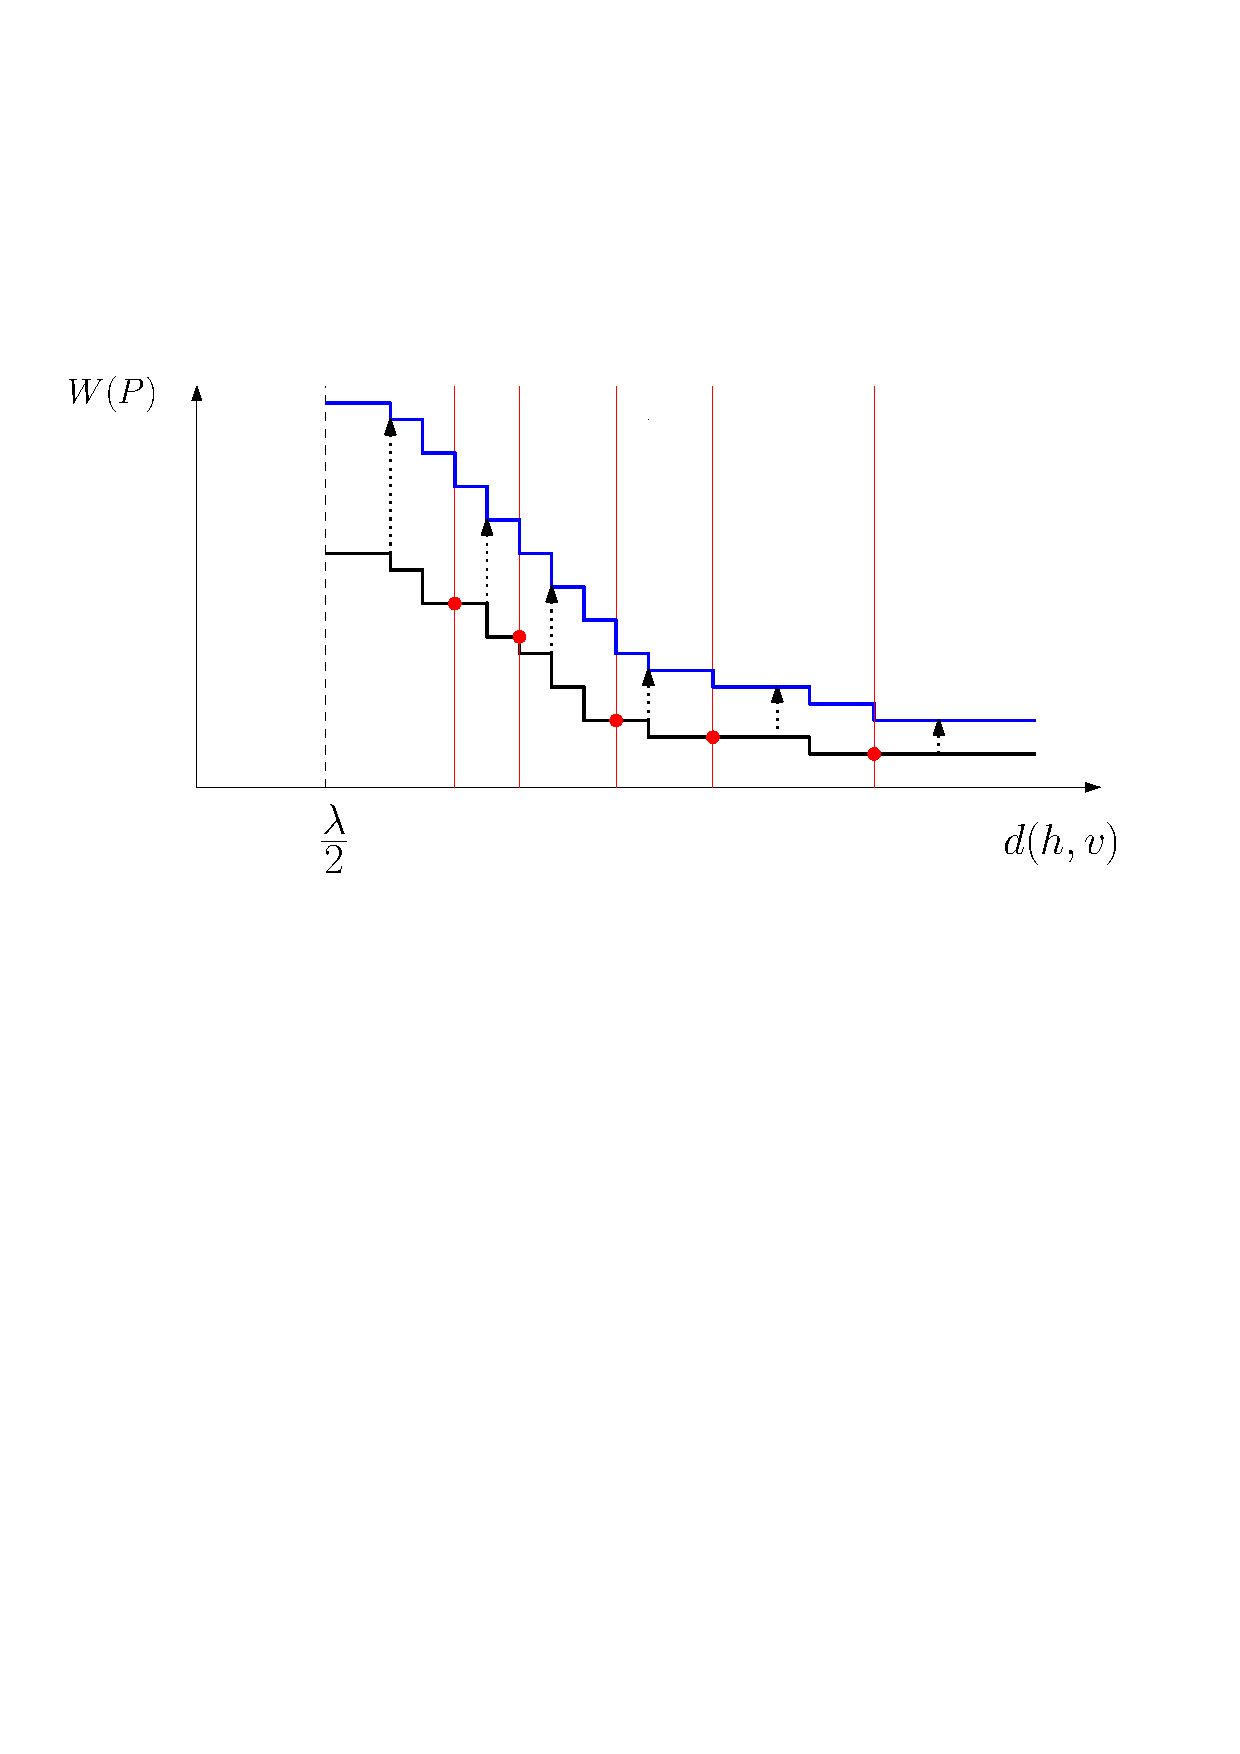
\includegraphics[scale=.55]{new_polyline_second_half}
\end{center}
\caption{Constructing the second half of the polyline $p$ (in blue). The black polyline is $p_2$. The breakpoints inserted from $p_1$ are in red. In each interval (between consecutive red lines) we raise the polyline by the value in $p_1$.
\label{figure of constructing the second half of the polyline}}
\end{figure}

\begin{figure}[h]
\begin{center}
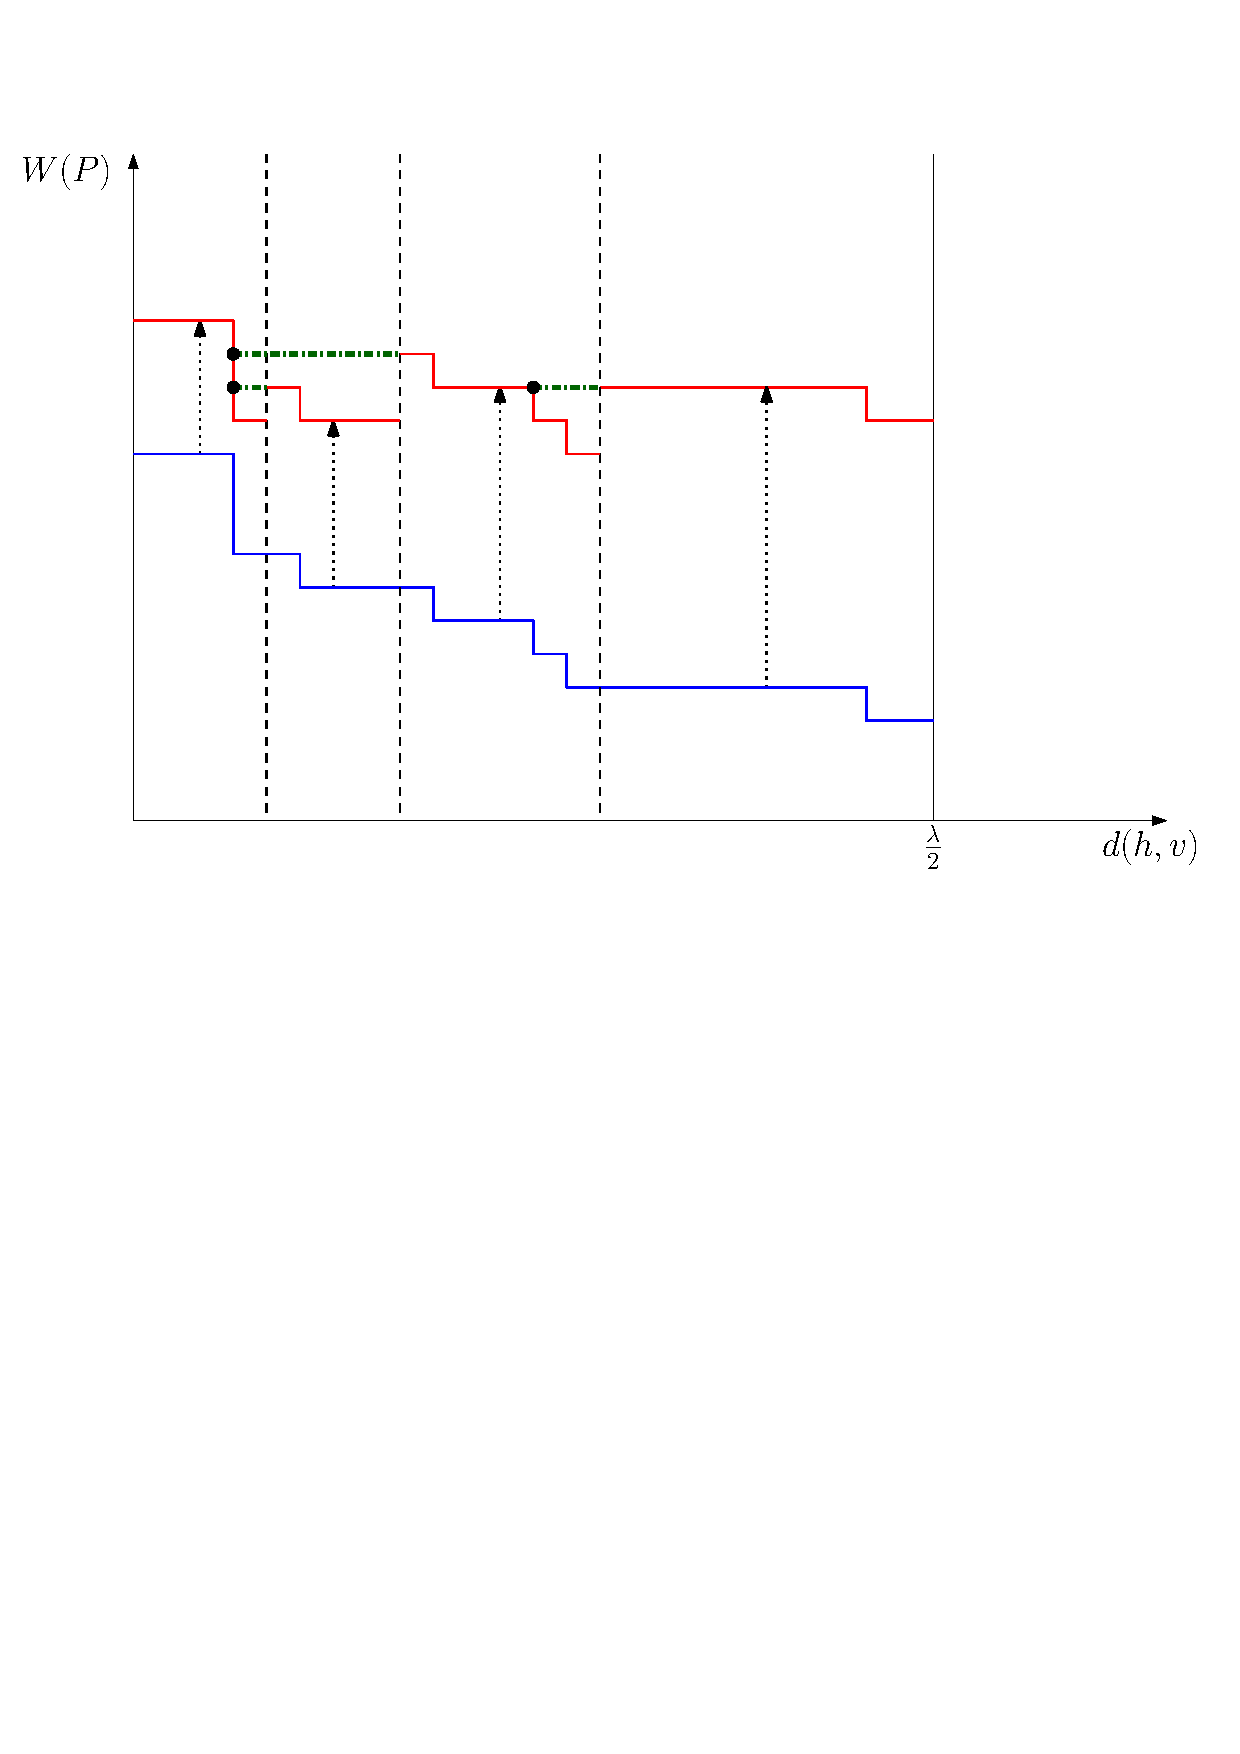
\includegraphics[scale=0.6]{polyline_first_half_construction_case2}
\end{center}
\caption{Case II of constructing the first half of the polyline. The first half of $p_2$ is in blue. The vertical black dashed lines are the breakpoints of $p_1$. We increase the values of $p_{2}$ and obtain the red polyline, which is not monotone. To make it monotone, we delete all the breakpoints below the green intervals, which are found with value predecessor queries (the results of these queries are the bold points).\label{figure of the second case in the construction of the first half of the polyline}
}
\end{figure}


\begin{figure}[ht]
\begin{center}
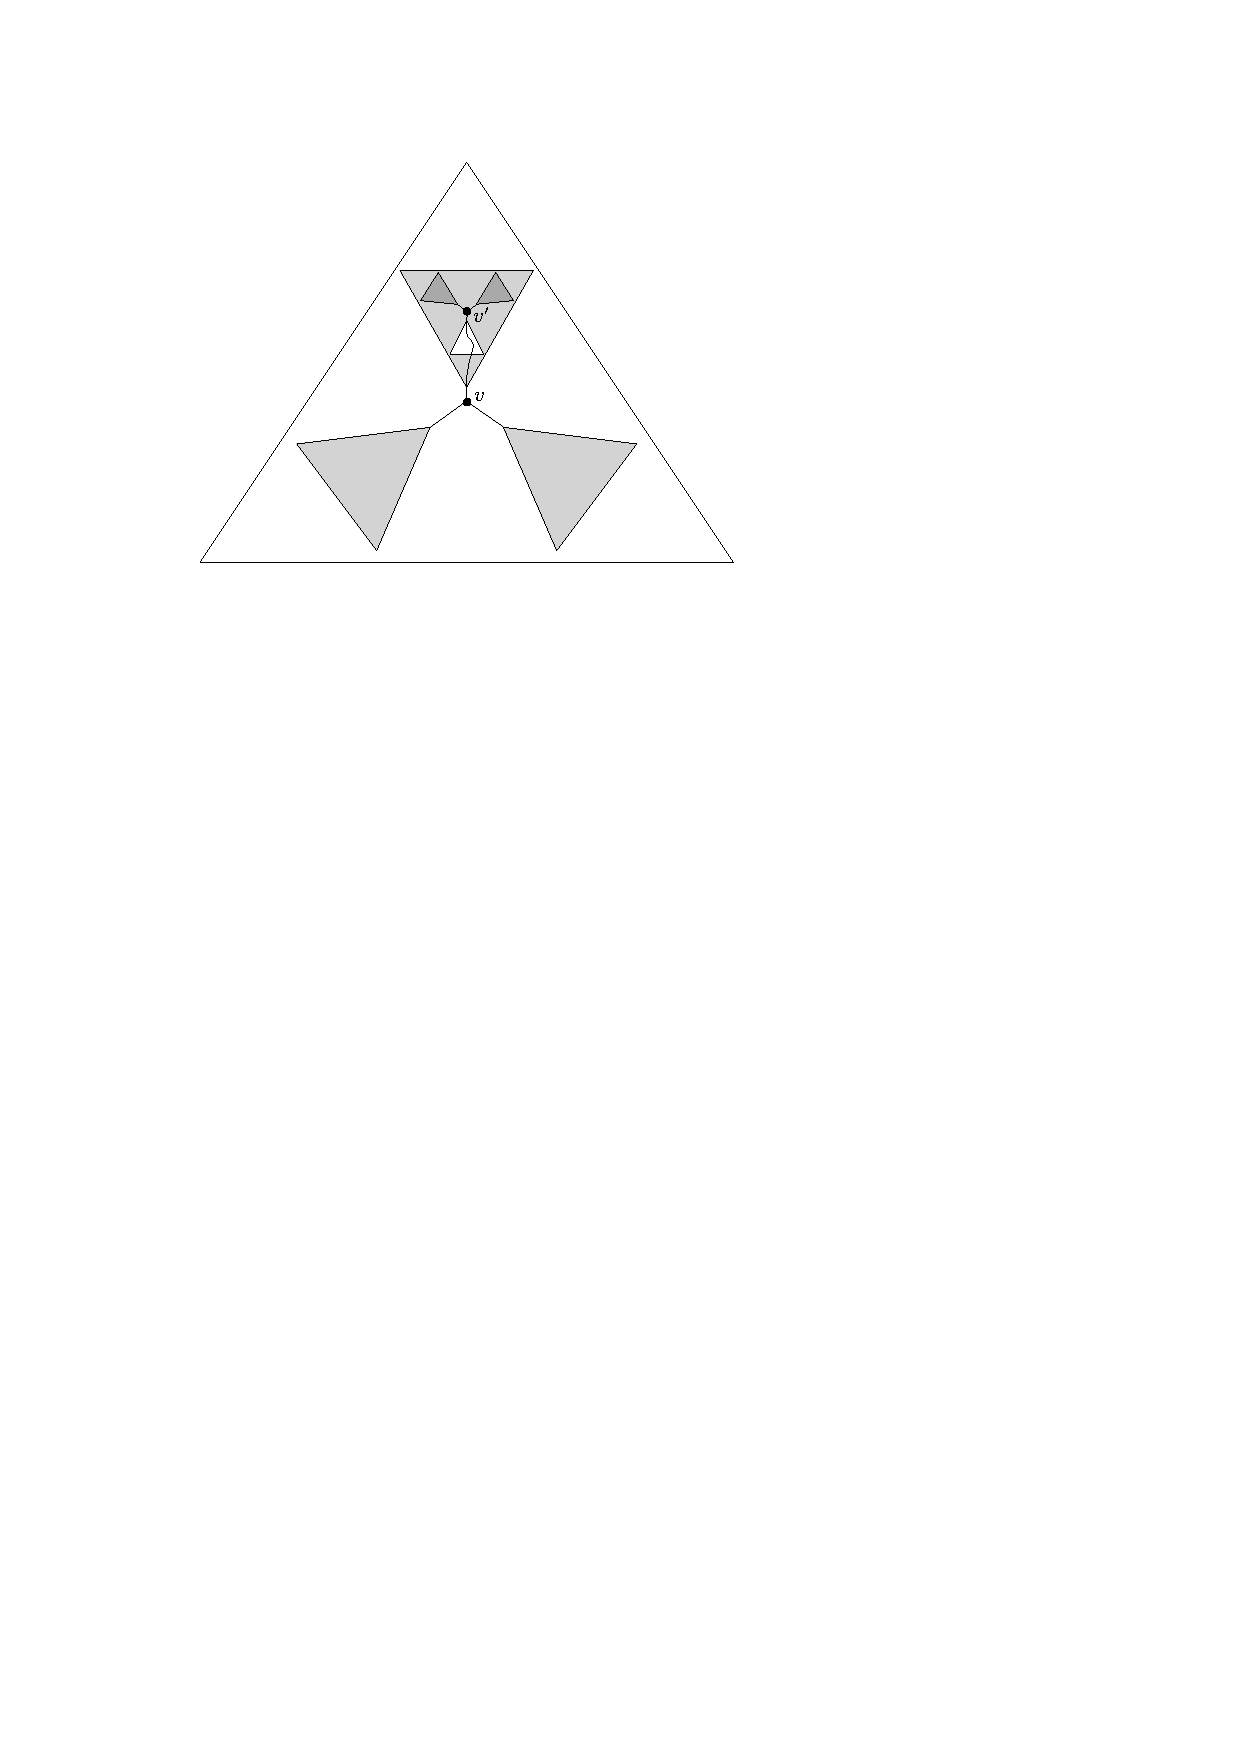
\includegraphics[scale=1]{centroid}
\end{center}
\caption{A single step in the centroid decomposition. Removing $v$ splits $T$ into three pieces, s.t. none of them has more than $\frac{|T|}{2}$ nodes. The white piece is problematic, since the paths from its nodes to $v$ do not pass through the inner centroid $v'$.}
\end{figure}


\begin{figure}[h]
\begin{center}
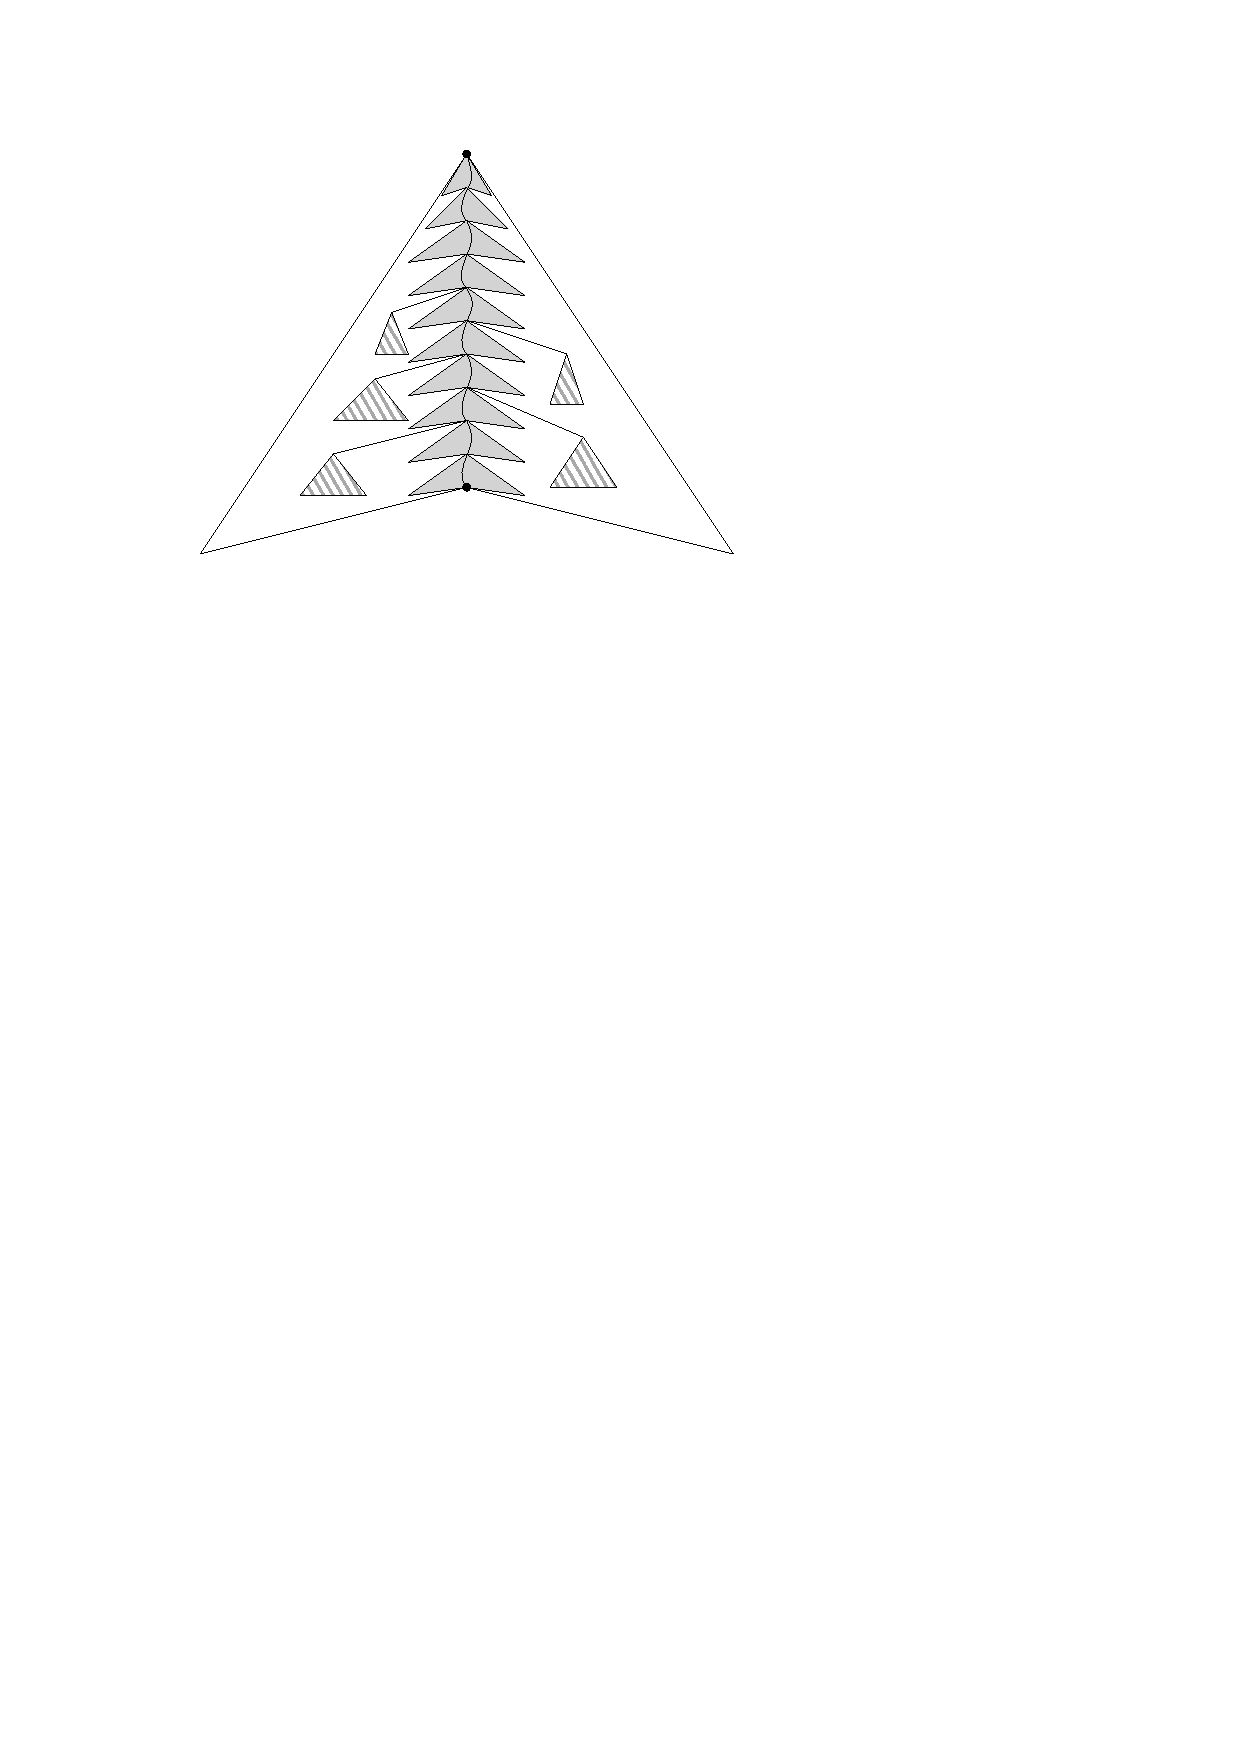
\includegraphics[scale=1]{refinement}
\end{center}
\caption{A large fragment containing a number of smaller fragments. The small fragments on the spine are gray, and the subtrees hanging off of the spine are black (each of them may contain many small fragments). %We start by reducing the hanging subtrees to just two nodes, then handle the small active fragments on the spine, and finally reduce the entire large fragment to one caterpillar and process it. 
\label{figure of small fragments inside a large fragment}}
\end{figure}


\end{document}

